\documentclass[12pt, a4paper]{article}

% ── PAQUETES ─────────────────────────────────────────────────
% Los paquetes amplían las capacidades de LaTeX.
% Se cargan en el "preámbulo" (antes de \begin{document}).

\usepackage[utf8]{inputenc}       % Permite tildes y ñ
\usepackage[spanish]{babel}       % Idioma español (guiones, fechas, etc.)
\usepackage{geometry}             % Control de márgenes
\usepackage{graphicx}             % Para insertar imágenes
\usepackage{setspace}             % Control de interlineado
\usepackage{hyperref}             % Links clicables (índice, URLs)
\usepackage{xcolor}               % Colores personalizados
\usepackage{listings}
\usepackage{tcolorbox}
\usepackage{amsmath}
\usepackage{float}
\usepackage{booktabs}
\usepackage{subcaption}
\usepackage{chngcntr}
\usepackage{array}
\usepackage{tabularx}
\usepackage{ragged2e}

\counterwithin{figure}{subsection}
\tcbuselibrary{listings, skins}

\newtcblisting{terminal}{
    colback   = black,           % fondo negro
    colframe  = gray!50,         % borde gris
    coltitle  = black,           % título en blanco
    coltext   = green!70!white,  % texto verde (estilo terminal clásica)
    title     = Terminal,
    fonttitle = \bfseries\small,
    listing only,
    listing options = {
        basicstyle = \ttfamily\small\color{green!70!white},
        breaklines = true,
    }
}

\lstset{
    basicstyle    = \ttfamily\small,   % fuente monoespaciada
    keywordstyle  = \color{blue},      % palabras clave en azul
    commentstyle  = \color{gray},      % comentarios en gris
    stringstyle   = \color{orange},    % strings en naranja
    numbers       = left,              % números de línea a la izquierda
    frame         = single,            % recuadro alrededor del bloque
    breaklines    = true,              % corta líneas largas automáticamente
}

\newcommand{\tema}{Python Fixed Point}
\newcommand{\titulotrabajo}{Informe}
\newcommand{\autor}{Alfici, Facundo Ezequiel}
\newcommand{\documento}{44012327}
\newcommand{\curso}{PROCOM}
\newcommand{\fundacion}{Fundación Fulgor}
\newcommand{\fecha}{\today}

% ── INICIO DEL DOCUMENTO ─────────────────────────────────────
% Todo lo visible va DENTRO de este entorno
\begin{document}

% Quitamos la numeración en la carátula
\thispagestyle{empty}

% ── CARÁTULA ─────────────────────────────────────────────────
\begin{center}   % Entorno para centrar contenido

    % --- Encabezado institucional ---
    {\Large \textbf{\fundacion}}\\[0.3cm]      % \\ fuerza un salto de línea                 % [0.2cm] = espacio extra después
    {\large \curso}

    \vspace{1.5cm}   % Espacio vertical de 1.5 cm

    % --- Logo (opcional) ---
    % Descomenta las 2 líneas siguientes si tenés un logo guardado
    % \includegraphics[width=0.25\textwidth]{logo.png}
    % \vspace{1cm}

    \hrule height 1pt   % Línea horizontal
    \vspace{0.4cm}

    % --- Título del trabajo ---
    {\LARGE \textbf{\titulotrabajo}}\\[0.3cm]
    {\large \tema}

    \vspace{0.4cm}
    \hrule height 1pt

    \vspace{2.5cm}

    % --- Datos del alumno ---
    % Tabla simple de 2 columnas: etiqueta y valor
    \begin{tabular}{r l}   % r = columna alineada a la derecha, l = izquierda
        \textbf{Autor:}   & \autor\\[0.2cm]
        \textbf{Documento:}  & \documento\\[0.2cm]
        \textbf{Docentes:} &  Ariel Pola, Santiago Garaventta Pascual y Agustín Pesce\\
    \end{tabular}

    \vspace{3cm}

    % --- Fecha ---
    {\large \fecha}

\end{center}

% Salto de página → el informe real comienza en la siguiente hoja
\newpage

% ── EJEMPLO DE PRIMERA SECCIÓN (para no dejar el doc vacío) ──
\tableofcontents   % Genera el índice automáticamente
\newpage


%Cuerpo del informe

\section{Introducción}
En este informe se aplicarán los conceptos de Aritmética de punto fijo utilizando la clase \textbf{fixedInt.py} con el fin de
familiarizarse con el uso de python para el cálculo y representación de las respuestas de filtros propuestos.
El ejercicio consta de 5 consignas, donde se pide aplicar los conceptos mencionados anteriormente sobre el filtro \textit{Raised Cosine}
del código en python proveniente del archivo \textbf{tx\_rcosine\_procom.py}. Los puntos a desarrollar se listan a continuación.
\begin{enumerate}
    \item Generar tres filtros con rolloff [0.0,0.5,1.0] en punto flotante con NBaud = 16,
    FBaud =1G y OS = 8.
    \item Graficar la respuesta al impulso y frecuencia.
    \item Graficar la convolución de los tres filtros con los símbolos a transmitir y la constelación buscando la fase óptima.
    \item Sobre cada filtro aplicar las siguiente cuantizaciones: S(8,7) truncado, S(8,7) redondeo,
    S(3,2) truncado, S(3,2) redondeo, S(6,4) truncado y S(6,4) redondeo. En todos los
    casos considerar saturación.
    \item Realizar con los nuevos filtros las gráficas anteriores y comparar resultados.
\end{enumerate}

\newpage

\section{Desarrollo}

\subsection{Generación de filtros Raised Cosine}
Comenzando con el desarollo, se pide generar tres filtros con diferentes valores de rolloff (exceso de ancho de banda) para punto flotante.
La respuesta al impulso se puede ver en la siguiente figura.
\begin{figure}[H]
    \centering
    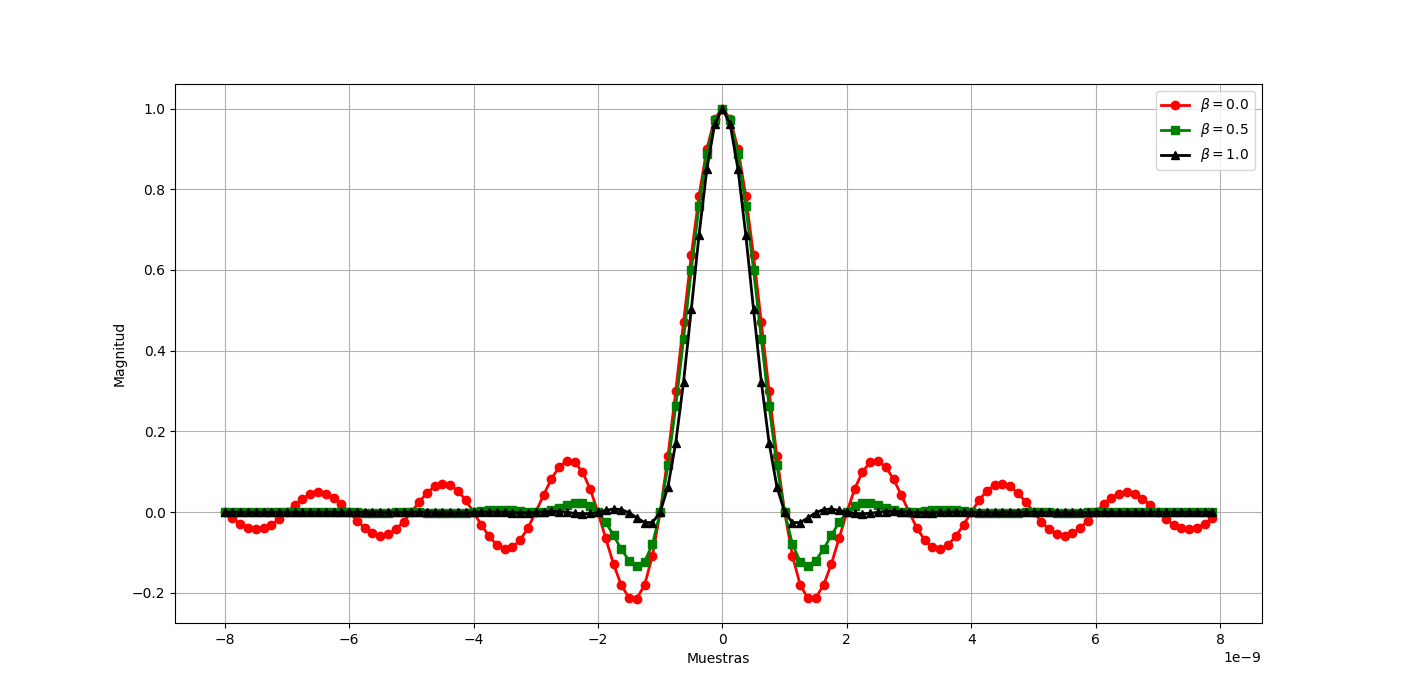
\includegraphics[width=1\textwidth]{imagenes_FP/rta_imp_1.png}
    \caption{Respuesta al Impulso de los filtros combinados}
    \label{fig:rta_imp_1}
\end{figure}
En la figura \ref{fig:rta_imp_1} se puede observar la clara diferencia en la respuesta al impulso de los filtros, donde según el valor de rolloff, el filtro
responderá de manera más o menos ondulatoria, siendo el filtro con el rolloff de 1 la respuesta con menor sobreoscilación.

De igual manera, se graficó la respuesta en frecuencia de los filtros, lo que se muestra en la siguiente figura.
\begin{figure}[H]
    \centering
    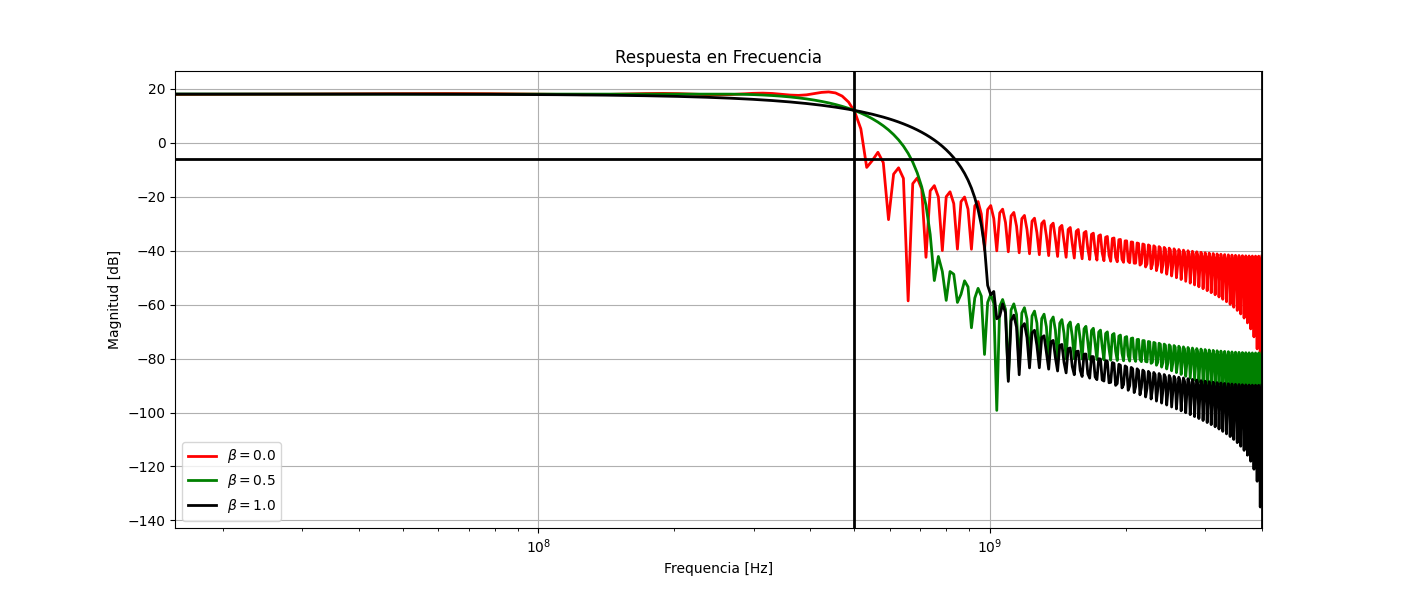
\includegraphics[width=1\textwidth]{imagenes_FP/rta_freq_1.png}
    \caption{Respuesta en Frecuencia de los filtros combinados}
    \label{fig:rta_freq_1}
\end{figure}
Donde se puede ver representada la clara diferencia entre las respuestas en frecuencia según el coeficiente de rolloff.

Algunas cosas importantes a analizar con el fin de entender lo que se ve en la figura \ref{fig:rta_freq_1} vienen dadas por el \textbf{eje} dibujado
por las lineas negras. Este eje nos muestra el punto donde cada filtro presenta su punto de \textbf{amplitud media} para el eje horizontal y la \textbf{frecuencia
de corte} para el eje vertical. Se llegó a esta conclusión analizando el código provisto.

La figura \ref{fig:rta_freq_1} muestra que la frecuencia de corte del filtro es \textit{independiente del factor de rolloff}, dado que los tres filtros
se intersectan con el eje vertical en el mismo punto. Por otra parte, \textit{el punto de amplitud media de cada uno varía significativamente}, de tal manera que
para un rolloff más cercano a 0, el punto de amplitud media se encontrará en una frecuencia menor.

Consiguientemente, se graficó la convolución de los tres filtros.

\begin{figure}[H]
    \centering
    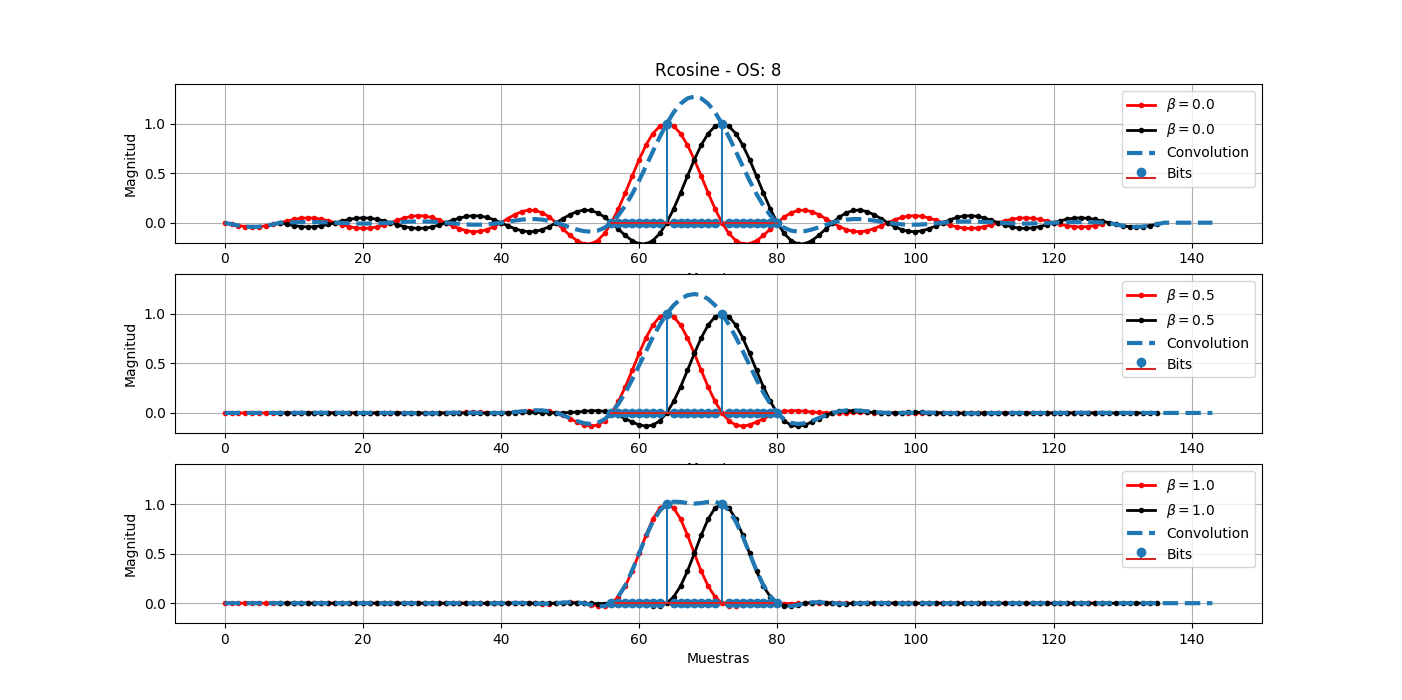
\includegraphics[width=1\textwidth]{imagenes_FP/os_effect_1.png}
    \caption{Convolución de los filtros}
    \label{fig:os_effect_1}
\end{figure}

Finalmente, se tienen los símbolos a transmitir, los diagramas de ojo y las constelaciones de los mismos.
Estos gráficos se realizaron sin modificaciones previas, con el fin de remarcar la importancia del offset para la constelación.

\begin{figure}[H]
    \centering
    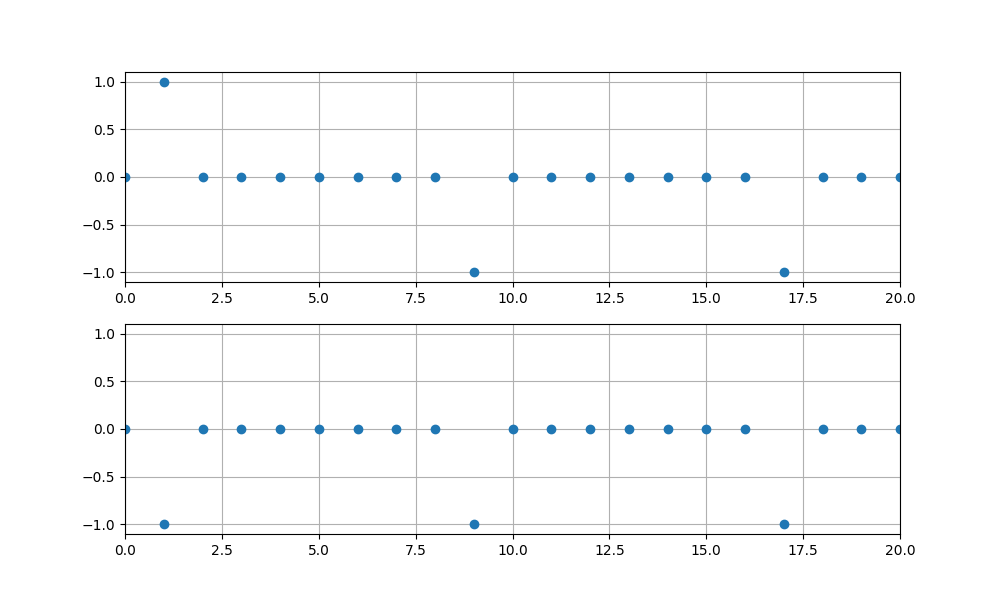
\includegraphics[width=1\textwidth]{imagenes_FP/simbols1.png}
    \caption{Secuencia de Símbolos}
    \label{fig:simbols_transmitted1}
\end{figure}

\begin{figure}[H]
    \centering
    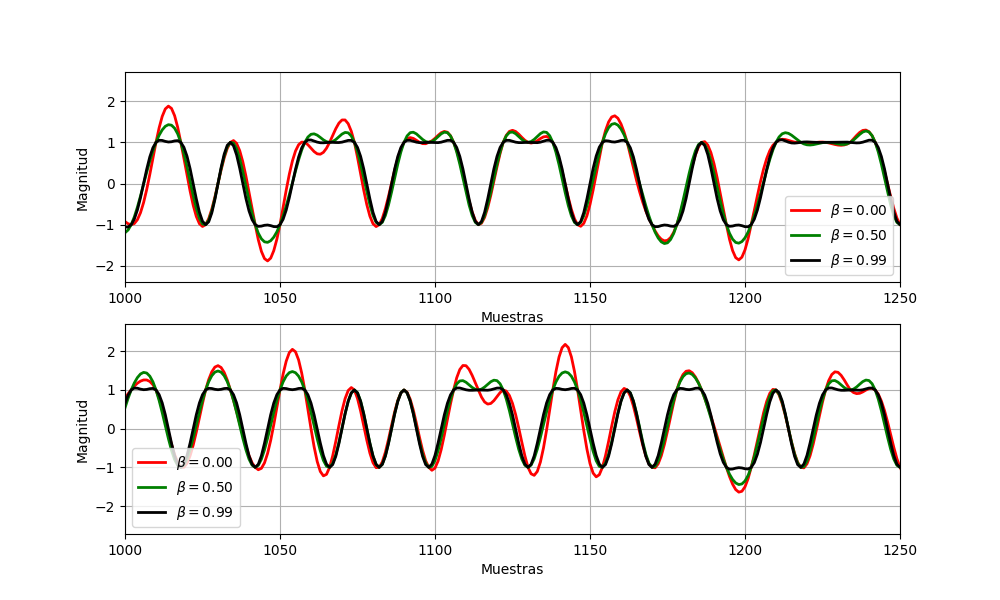
\includegraphics[width=1\textwidth]{imagenes_FP/simbols_in_out1.png}
    \caption{Señal recibida}
    \label{fig:simbols_in_out1}
\end{figure}

Como es visible en la figura \ref{fig:simbols_in_out1}, la interferencia entre cada símbolo es mucho mayor para los filtros donde
el factor de rolloff es más cercano a 0. Esto también es posible de ver en los diagramas de ojo, donde para el filtro con $\alpha=0$ la interferencia
entre símbolos es mucho mayor, lo que hace que el ojo se vea más cerrado. 

\begin{figure}[H]
    \centering

    \begin{subfigure}{0.49\textwidth}
        \centering
        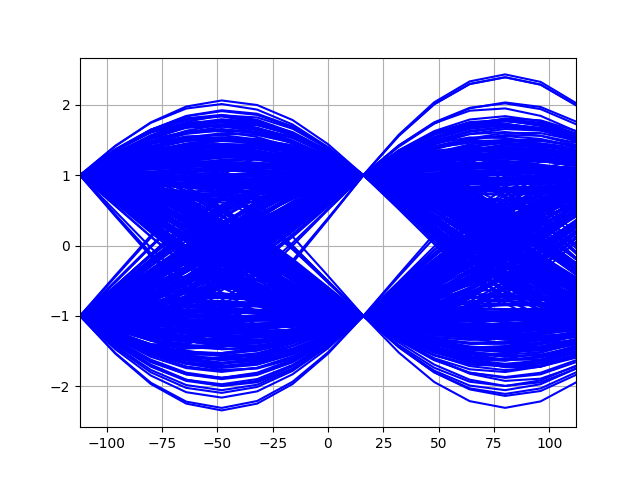
\includegraphics[width=\linewidth]{imagenes_FP/eye_d_filter0i.png}
    \end{subfigure}
    \hfill
    \begin{subfigure}{0.49\textwidth}
        \centering
        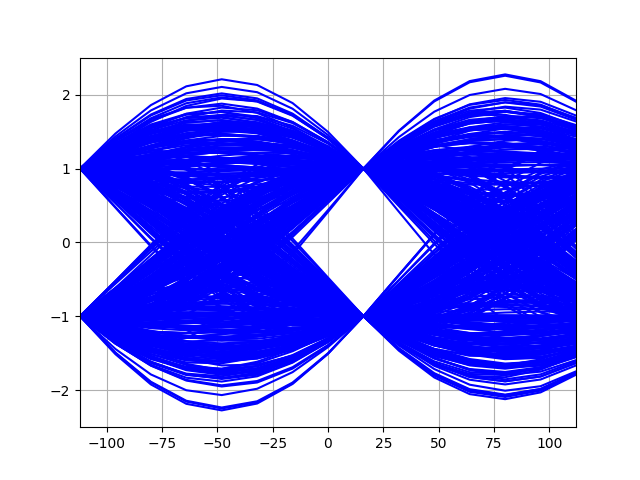
\includegraphics[width=\linewidth]{imagenes_FP/eye_d_filter0q.png}
    \end{subfigure}

    \caption{Diagrama de ojo de fase y cuadratura del filtro con $\alpha=0$ }
    \label{fig:eye_d_filter0}
\end{figure}

\begin{figure}[H]
    \centering

    \begin{subfigure}{0.49\textwidth}
        \centering
        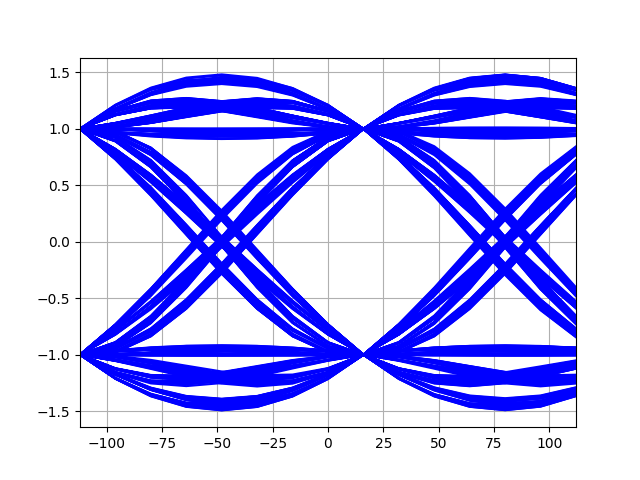
\includegraphics[width=\linewidth]{imagenes_FP/eye_d_filter1i.png}
    \end{subfigure}
    \hfill
    \begin{subfigure}{0.49\textwidth}
        \centering
        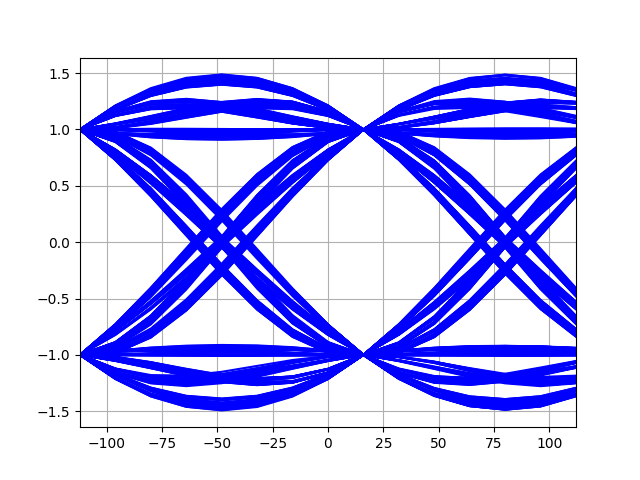
\includegraphics[width=\linewidth]{imagenes_FP/eye_d_filter1q.png}
    \end{subfigure}

    \caption{Diagrama de ojo de fase y cuadratura del filtro con $\alpha=0.5$ }
    \label{fig:eye_d_filter1}
\end{figure}

\begin{figure}[H]
    \centering

    \begin{subfigure}{0.49\textwidth}
        \centering
        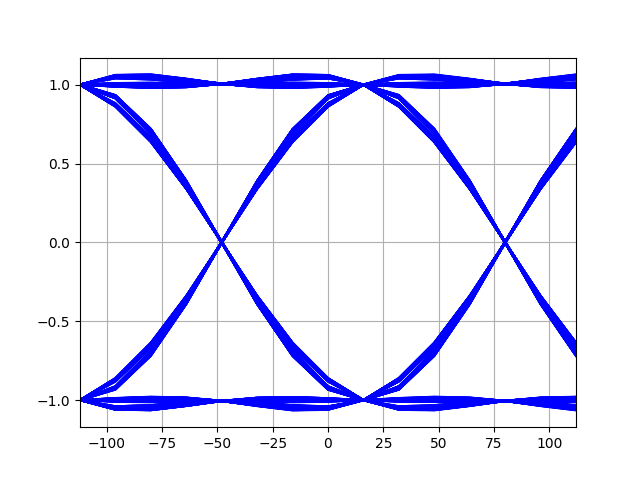
\includegraphics[width=\linewidth]{imagenes_FP/eye_d_filter2i.png}
    \end{subfigure}
    \hfill
    \begin{subfigure}{0.49\textwidth}
        \centering
        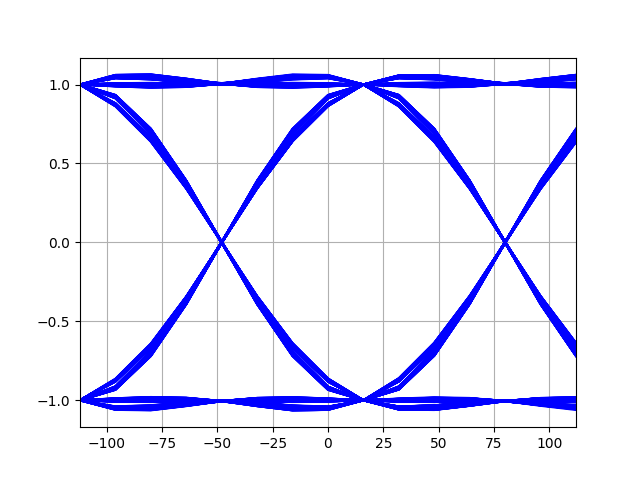
\includegraphics[width=\linewidth]{imagenes_FP/eye_d_filter2q.png}
    \end{subfigure}

    \caption{Diagrama de ojo de fase y cuadratura del filtro con $\alpha=1$ }
    \label{fig:eye_d_filter2}
\end{figure}
Ahora, viendo que la \textbf{interferencia entre símbolos (ISI)} es mucho mayor para filtros con menor rolloff, esto
nos podría guiar a que es mejor utilizar esta característica en todos los filtros, pero es un concepto erróneo.
Esto se debe a que, si bien la interferencia entre símbolos es prácticamente nula, se necesita un ancho de banda mayor,
lo que hace que se convierta en un juego de equilibrio entre interferencia y ancho de banda.

Lo que respecta a las constelaciones, se tienen las siguientes gráficas.

\begin{figure}[H]
    \centering

    \begin{subfigure}{0.32\textwidth}
        \centering
        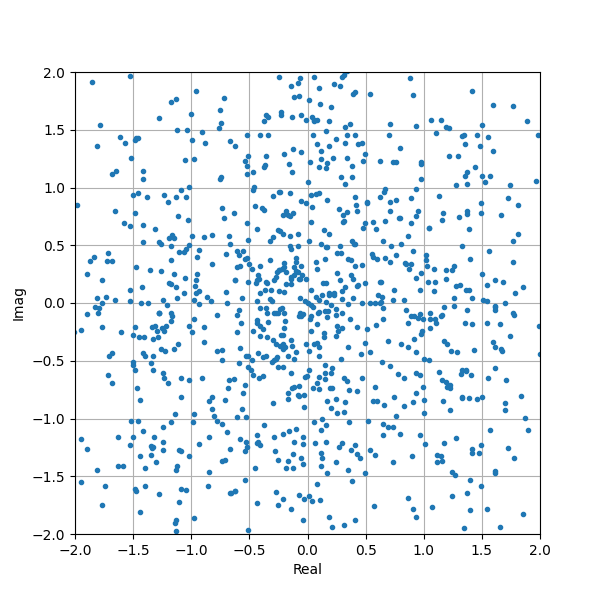
\includegraphics[width=\linewidth]{imagenes_FP/constelation_filter0.png}
        \caption{$\alpha=0$}
        \label{fig:constelation_filter0}
    \end{subfigure}
    \hfill
    \begin{subfigure}{0.32\textwidth}
        \centering
        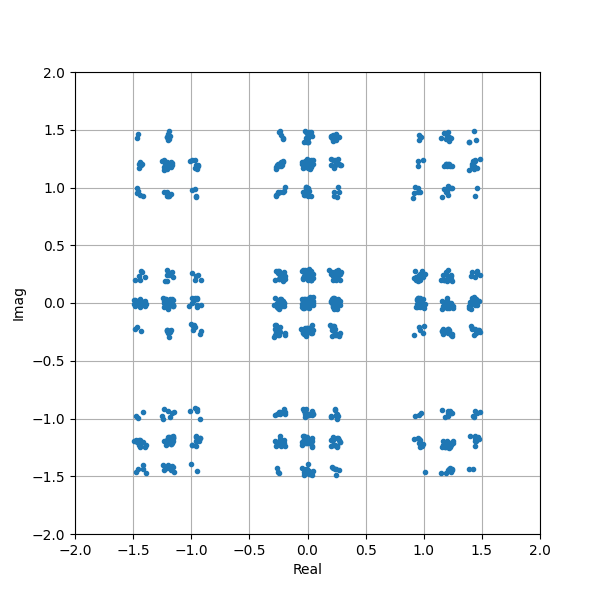
\includegraphics[width=\linewidth]{imagenes_FP/constelation_filter1.png}
        \caption{$\alpha=0.5$}
        \label{fig:constelation_filter1}
    \end{subfigure}
    \hfill
    \begin{subfigure}{0.32\textwidth}
        \centering
        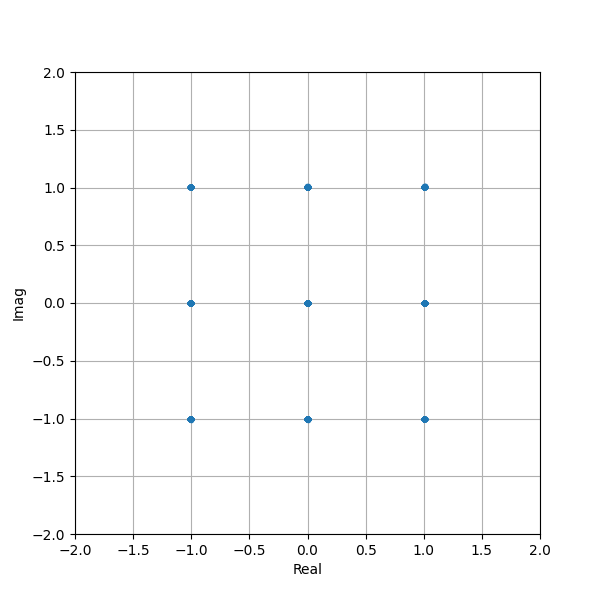
\includegraphics[width=\linewidth]{imagenes_FP/constelation_filter2.png}
        \caption{$\alpha=1$}
        \label{fig:constelation_filter2}
    \end{subfigure}
    \caption{Constelaciones de los filtros según el rolloff}
    \label{fig:constelations}
\end{figure}
Para todos los casos, vemos un problema clave en las constelaciones; El \textbf{offset.}

Es muy importante elegir correctamente el valor de \textbf{offset} para las gráficas generadas debido a que este valor nos permitirá
seleccionar el punto en el que se desea graficar la constelación, y, si el punto no es el óptimo,
la constelación se verá afectada en mayor o menor medida.

Para los casos actuales, se cambió el offset por defecto (2) a un valor óptimo (6), con el que se obtuvieron las siguientes capturas.

\begin{figure}[H]
    \centering

    \begin{subfigure}{0.32\textwidth}
        \centering
        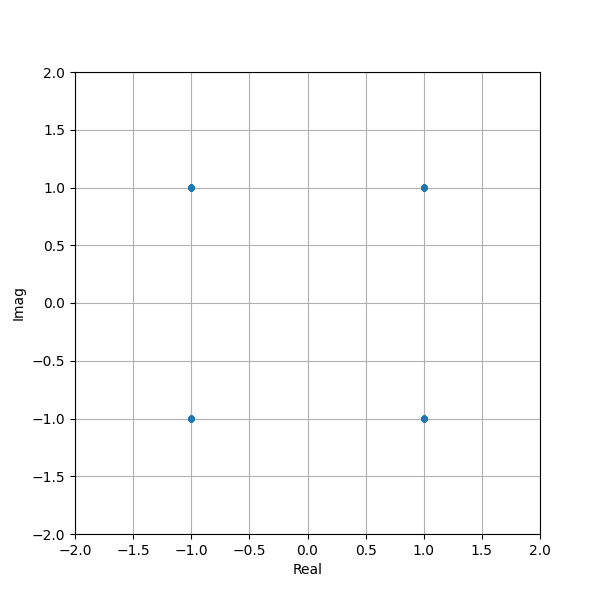
\includegraphics[width=\linewidth]{imagenes_FP/constelation_filter0_opt.png}
        \caption{$\alpha=0$}
        \label{fig:constelation_filter0_opt}
    \end{subfigure}
    \hfill
    \begin{subfigure}{0.32\textwidth}
        \centering
        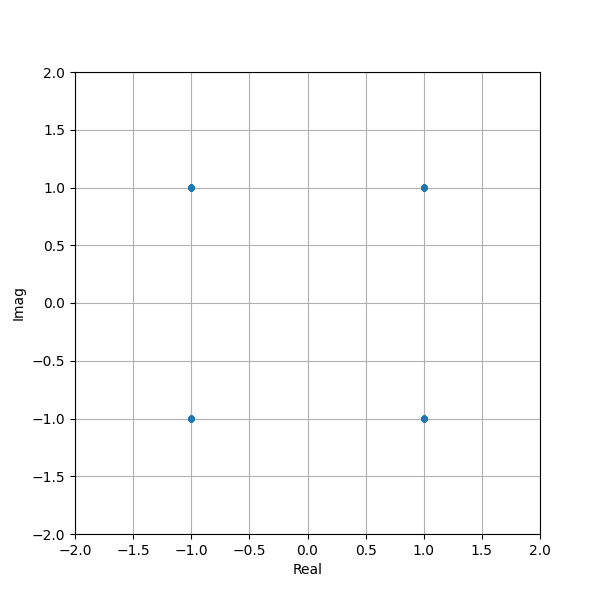
\includegraphics[width=\linewidth]{imagenes_FP/constelation_filter1_opt.png}
        \caption{$\alpha=0.5$}
        \label{fig:constelation_filter1_opt}
    \end{subfigure}
    \hfill
    \begin{subfigure}{0.32\textwidth}
        \centering
        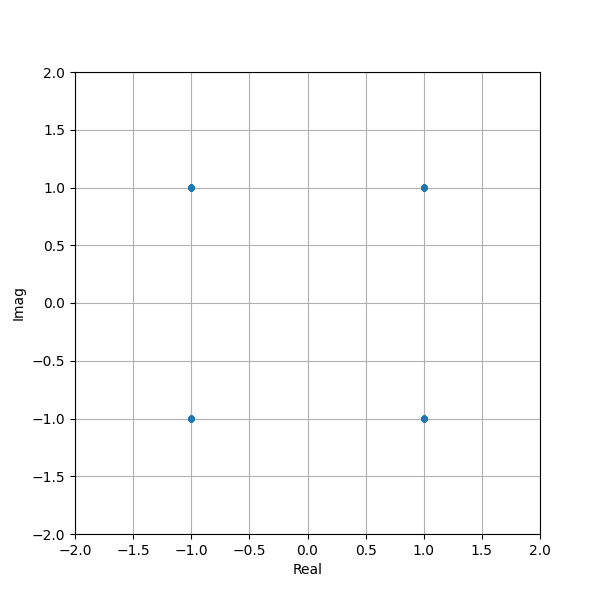
\includegraphics[width=\linewidth]{imagenes_FP/constelation_filter2_opt.png}
        \caption{$\alpha=1$}
        \label{fig:constelation_filter2_opt}
    \end{subfigure}
    \caption{Constelaciones de los filtros según el rolloff con fase óptima}
    \label{fig:constelations_opt}
\end{figure}
Donde se observa que la interferencia de la constelación es nula en todos los casos.

\subsection{Cuantización de los filtros generados}

Se pidió aplicar diferentes cuantizaciones a los filtros ya analizados, 
pero previamente es necesario explicar la forma en la que se aprovechó la clase \textit{fixedInt.py}.
Dentro de la clase se encuentra un método llamado \textit{arrayFixedInt()} el cual genera un arreglo con los coeficientes
ya tratados según los parámetros introducidos. Éste método permite generar coeficientes signed o unsigned, truncados o redondeados y saturados o wrapped.

Sabiendo la estructura del método, se generaron los coeficientes según la consigna para luego transformar su valor a float, con
el fin de trabajarlos mediante NumPy o para graficarlos.

\subsection{Cuantización S(8,7)}
Las gráficas estarán centradas principalmente en la convolución, el diagrama
de ojo, la respuesta al impulso, la respuesta en frecuencia y la constelación.
Los símbolos enviados no cambiarán por lo que no se graficarán. También es importante aclarar que las
comparaciones se harán en un subapartado externo.

\begin{figure}[H]
    \centering

    \begin{subfigure}{0.49\textwidth}
        \centering
        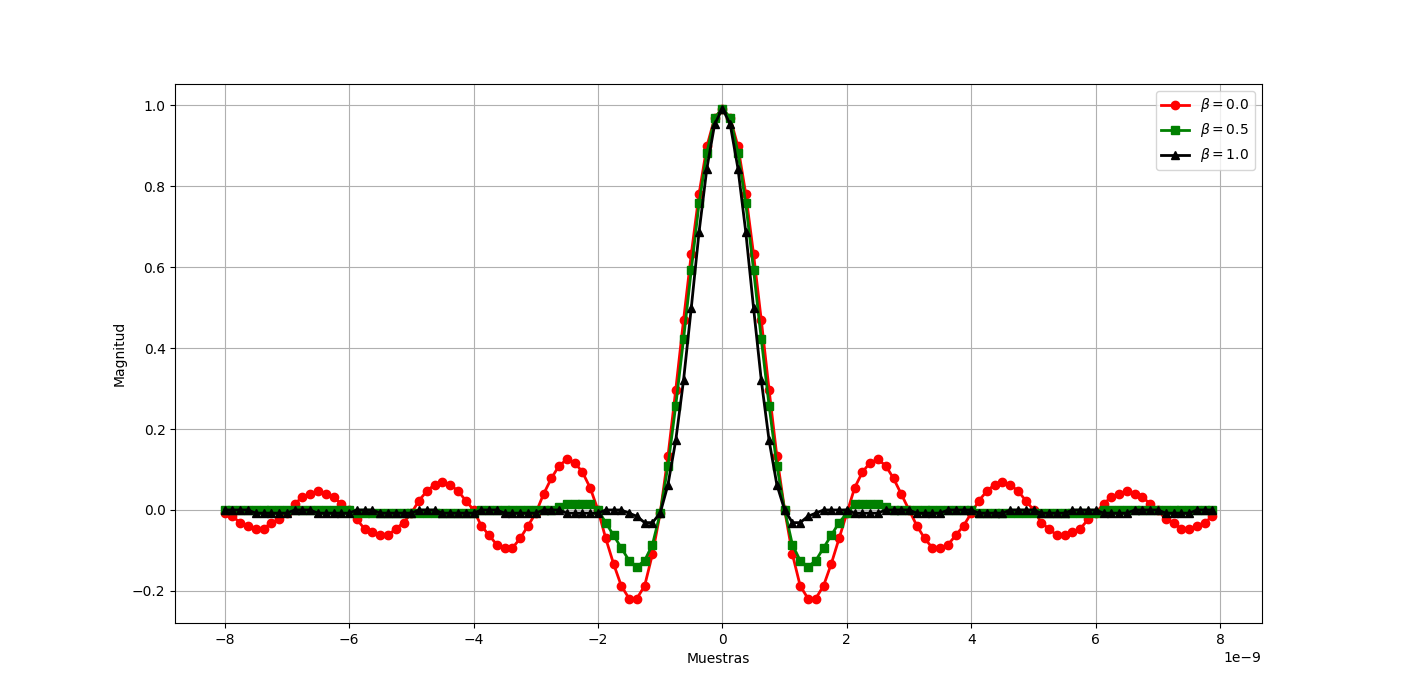
\includegraphics[width=\linewidth]{imagenes_FP/rta_imp_8,7_trunc.png}
        \caption{Respuesta al impulso según $\alpha$}
        \label{fig:rta_imp_8_7_trunc}
    \end{subfigure}
    \hfill
    \begin{subfigure}{0.49\textwidth}
        \centering
        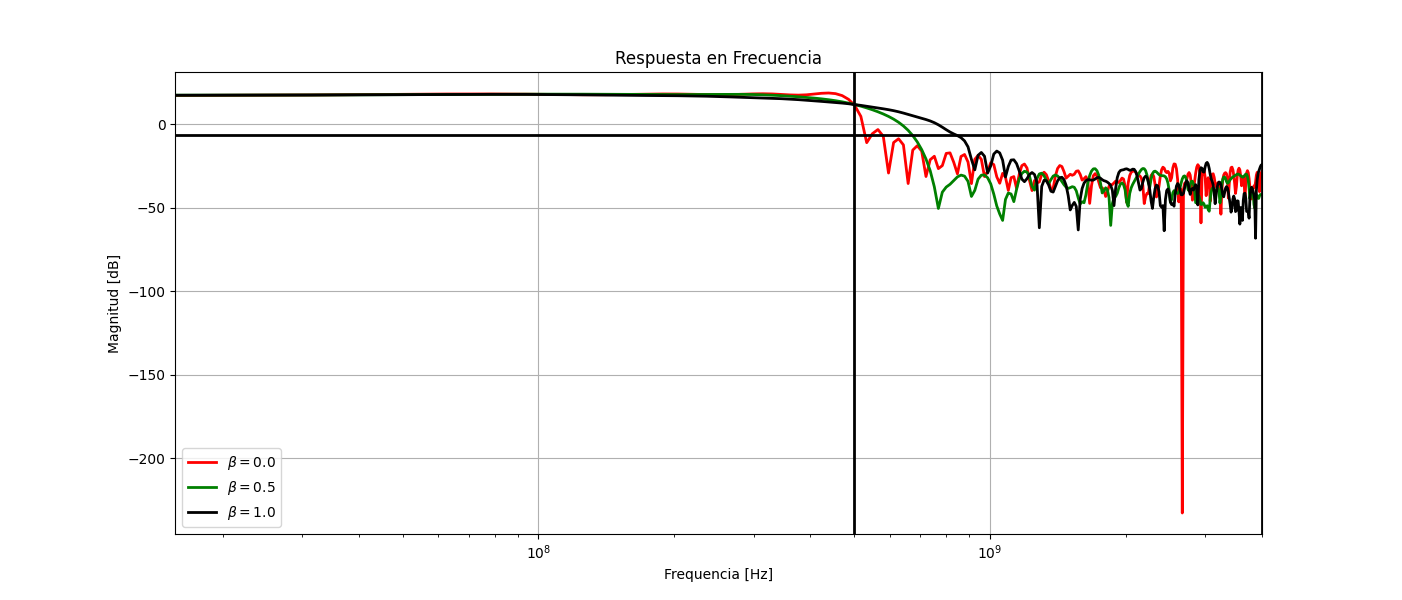
\includegraphics[width=\linewidth]{imagenes_FP/rta_freq_8,7_trunc.png}
        \caption{Respuesta en frecuencia según $\alpha$}
        \label{fig:rta_freq_8_7_trunc}
    \end{subfigure}
    \caption{Respuesta en tiempo y frecuencia S(8,7) truncado}
\end{figure}

\begin{figure}[H]
    \centering

    \begin{subfigure}{0.49\textwidth}
        \centering
        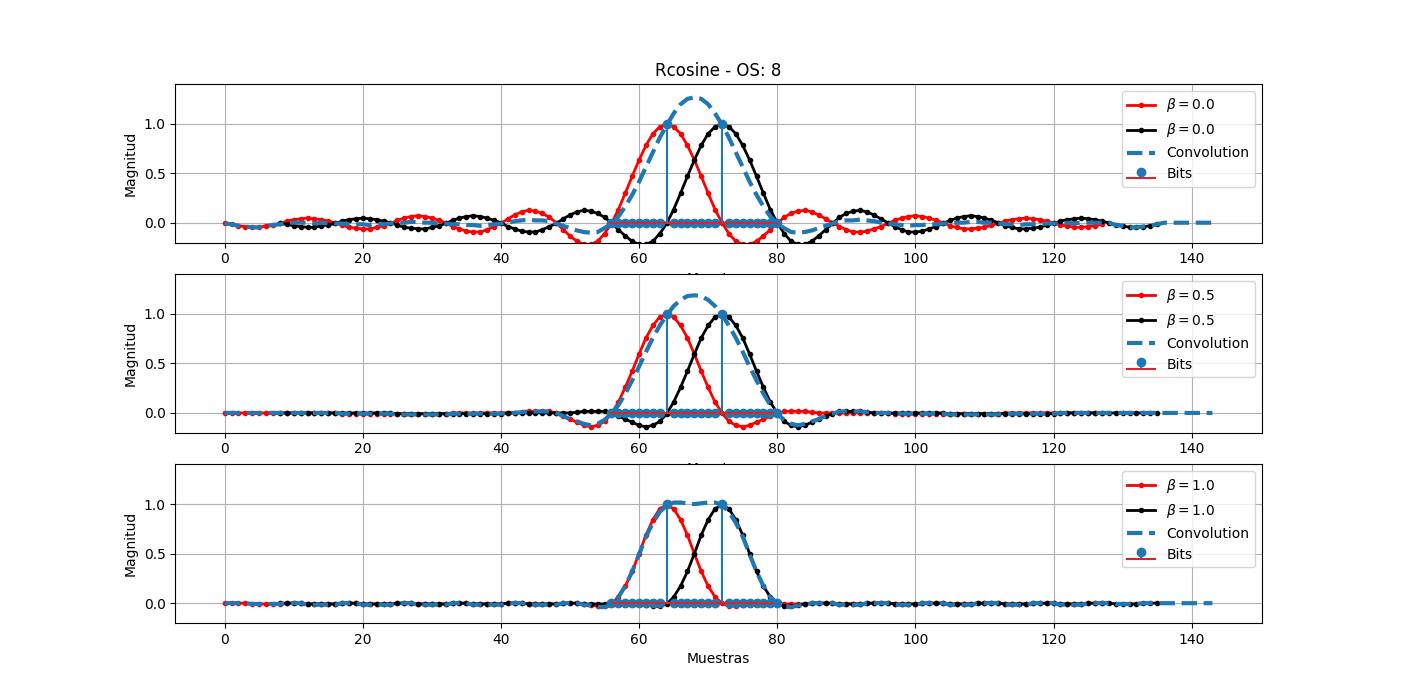
\includegraphics[width=\linewidth]{imagenes_FP/os_effect_8,7_trunc.png}
        \caption{Convolución según $\alpha$}
        \label{fig:os_effect_8_7_trunc}
    \end{subfigure}
    \hfill
    \begin{subfigure}{0.49\textwidth}
        \centering
        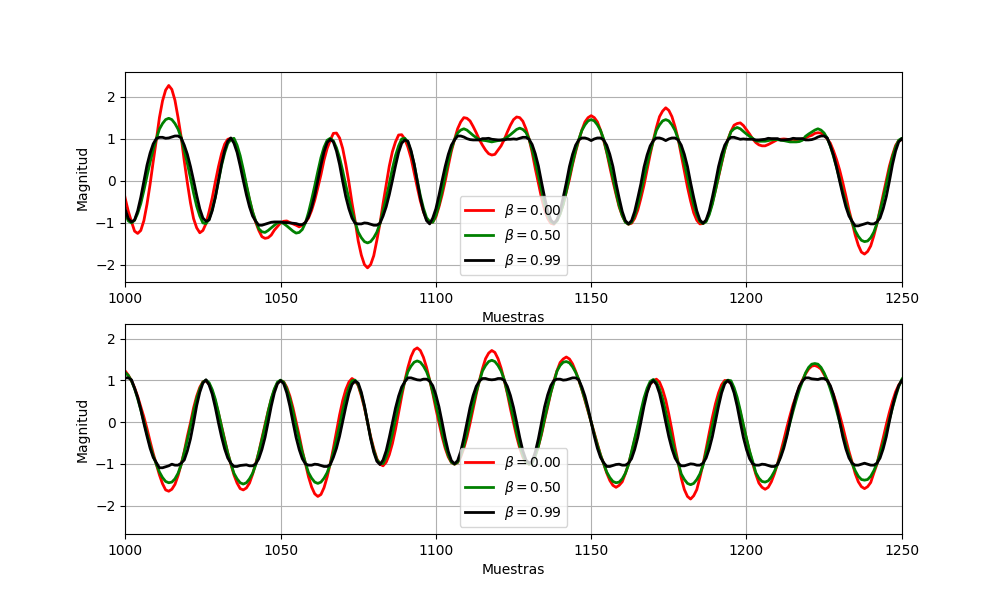
\includegraphics[width=\linewidth]{imagenes_FP/simbols_in_out8,7_trunc.png}
        \caption{Señal transmitida según $\alpha$}
        \label{fig:simbols_in_out8_7_trunc}
    \end{subfigure}
    \caption{Convolución y Transmisión S(8,7) truncado}
\end{figure}

\begin{figure}[H]
    \centering

    \begin{subfigure}{0.49\textwidth}
        \centering
        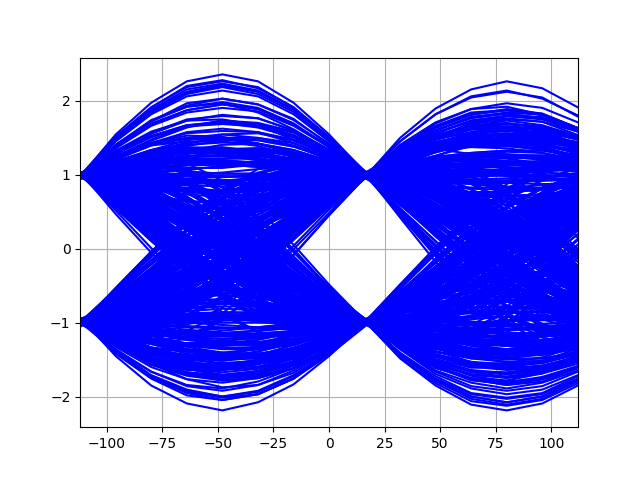
\includegraphics[width=\linewidth]{imagenes_FP/eye_d_filter0i8,7_trunc.png}
    \end{subfigure}
    \hfill
    \begin{subfigure}{0.49\textwidth}
        \centering
        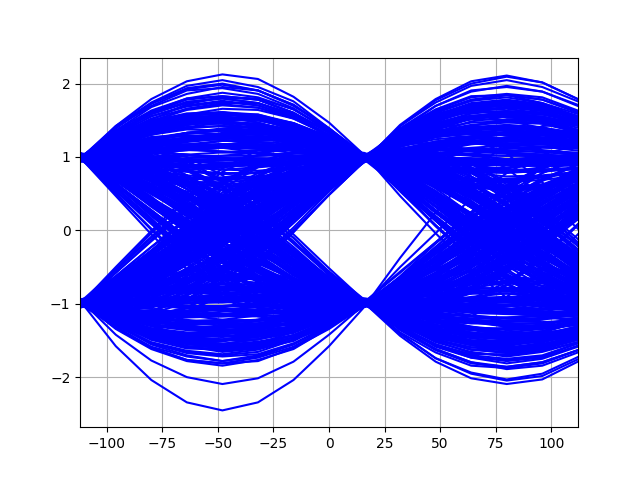
\includegraphics[width=\linewidth]{imagenes_FP/eye_d_filter0q8,7_trunc.png}
    \end{subfigure}
    \caption{Diagrama de ojo S(8,7) truncado con $\alpha=0$}
    \label{fig:eye_d_filter0q8_7_trunc}
\end{figure}

\begin{figure}[H]
    \centering

    \begin{subfigure}{0.49\textwidth}
        \centering
        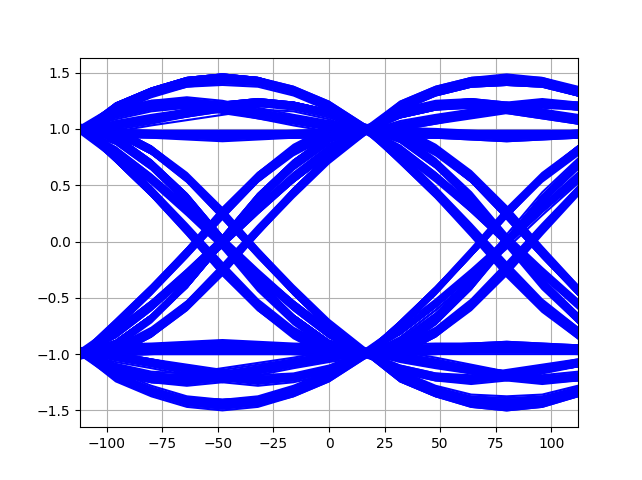
\includegraphics[width=\linewidth]{imagenes_FP/eye_d_filter1i8,7_trunc.png}
    \end{subfigure}
    \hfill
    \begin{subfigure}{0.49\textwidth}
        \centering
        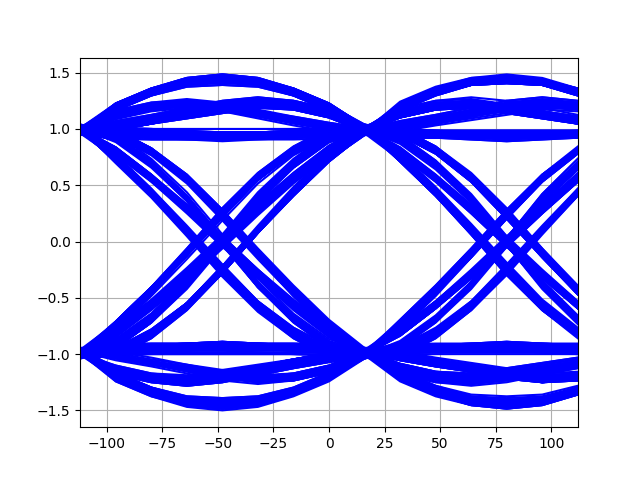
\includegraphics[width=\linewidth]{imagenes_FP/eye_d_filter1q8,7_trunc.png}
    \end{subfigure}
    \caption{Diagrama de ojo S(8,7) truncado con $\alpha=0.5$}
    \label{fig:eye_d_filter1q8_7_trunc}
\end{figure}

\begin{figure}[H]
    \centering

    \begin{subfigure}{0.49\textwidth}
        \centering
        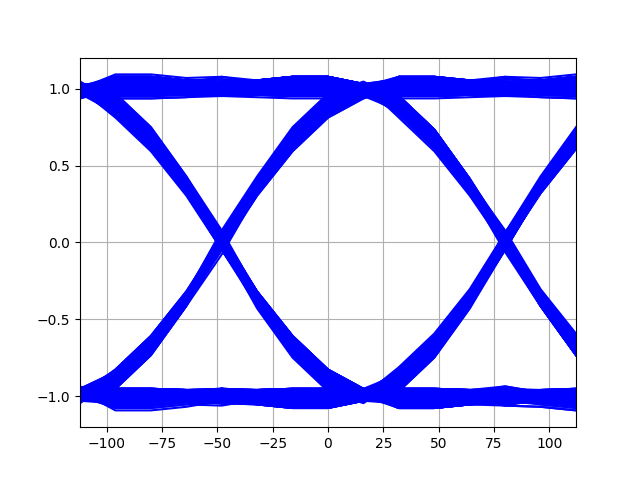
\includegraphics[width=\linewidth]{imagenes_FP/eye_d_filter2i8,7_trunc.png}
    \end{subfigure}
    \hfill
    \begin{subfigure}{0.49\textwidth}
        \centering
        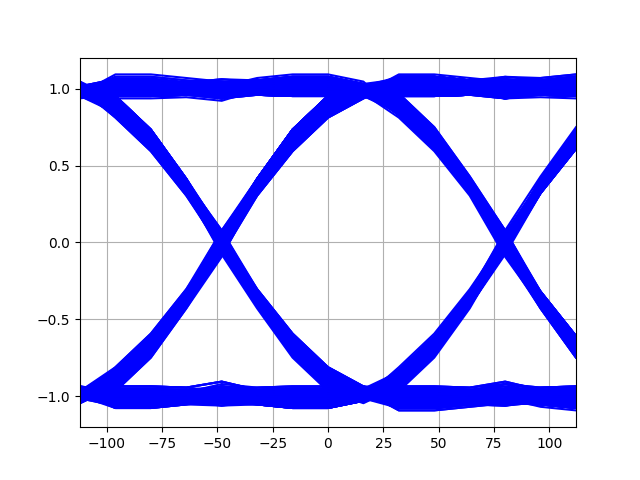
\includegraphics[width=\linewidth]{imagenes_FP/eye_d_filter2q8,7_trunc.png}
    \end{subfigure}
    \caption{Diagrama de ojo S(8,7) truncado con $\alpha=1$}
    \label{fig:eye_d_filter2q8_7_trunc}
\end{figure}

\begin{figure}[H]
    \centering

    \begin{subfigure}{0.32\textwidth}
        \centering
        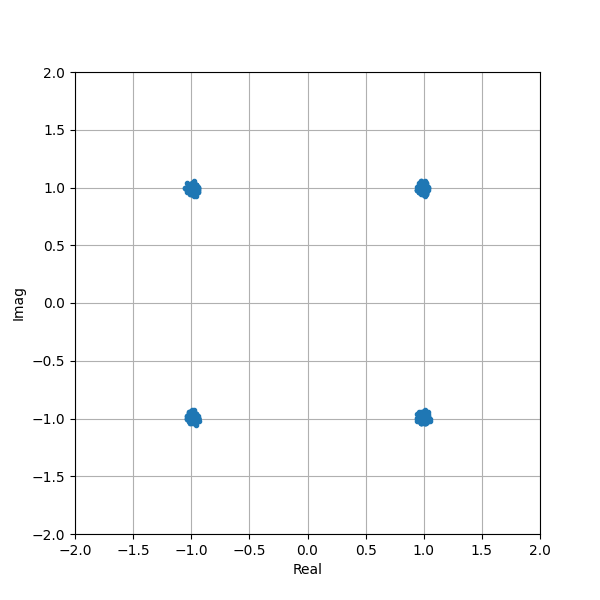
\includegraphics[width=\linewidth]{imagenes_FP/constelation_filter0_opt8,7_trunc.png}
        \caption{$\alpha=0$}
    \end{subfigure}
    \hfill
    \begin{subfigure}{0.32\textwidth}
        \centering
        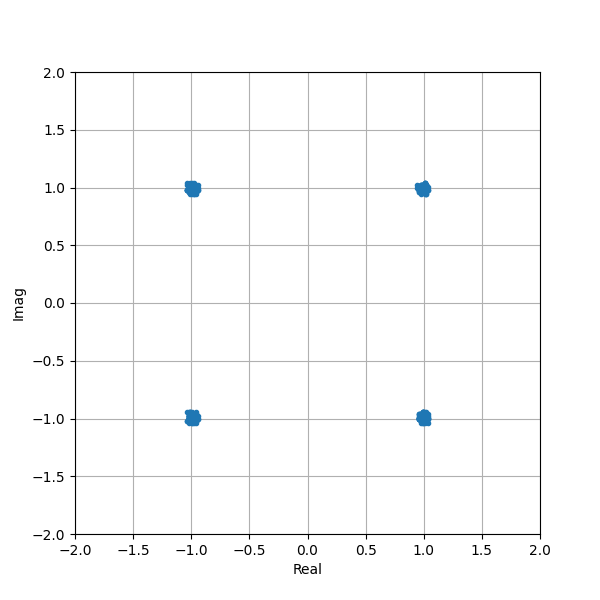
\includegraphics[width=\linewidth]{imagenes_FP/constelation_filter1_opt8,7_trunc.png}
        \caption{$\alpha=0.5$}
    \end{subfigure}
    \hfill
    \begin{subfigure}{0.32\textwidth}
        \centering
        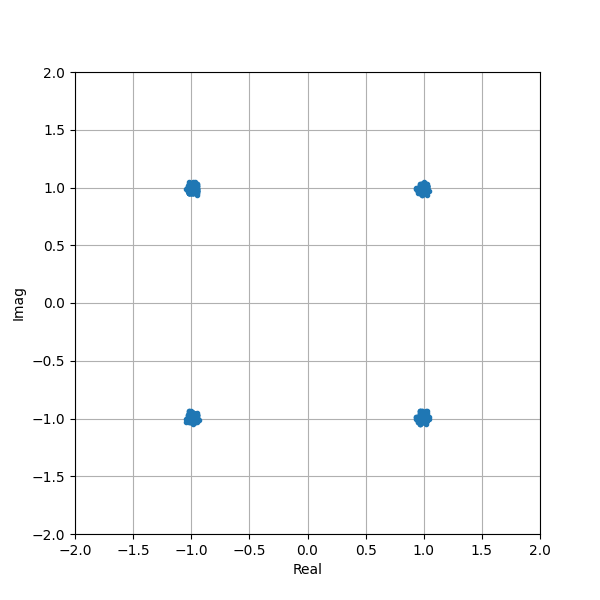
\includegraphics[width=\linewidth]{imagenes_FP/constelation_filter2_opt8,7_trunc.png}
        \caption{$\alpha=1$}
    \end{subfigure}
    \caption{Constelaciones según $\alpha$ para S(8,7) truncado}
    \label{fig:constelations_filters_opt8_7_trunc}
\end{figure}

De igual manera, se realizará el mismo procedimiento pero cuantizando con redondeo.
Para minizar la cantidad de imágenes presentadas, se omitirán en este caso la respuesta en tiempo y frecuencia,
la convolución y la señal transmitida debido a que la diferencia es mínima para ambas configuraciones.

\begin{figure}[H]
    \centering

    \begin{subfigure}{0.49\textwidth}
        \centering
        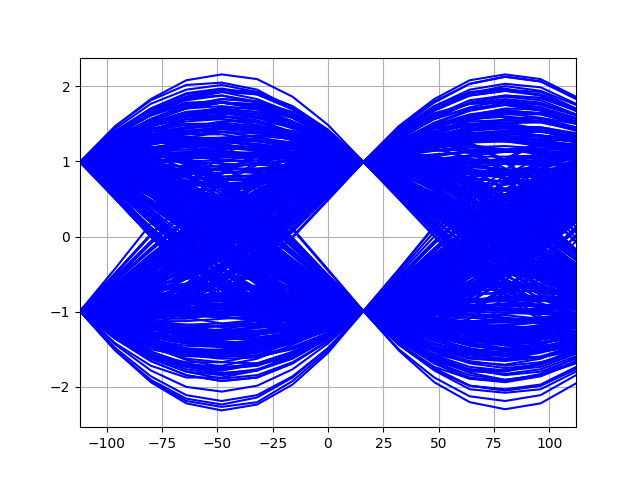
\includegraphics[width=\linewidth]{imagenes_FP/eye_d_filter0i8,7_round.png}
    \end{subfigure}
    \hfill
    \begin{subfigure}{0.49\textwidth}
        \centering
        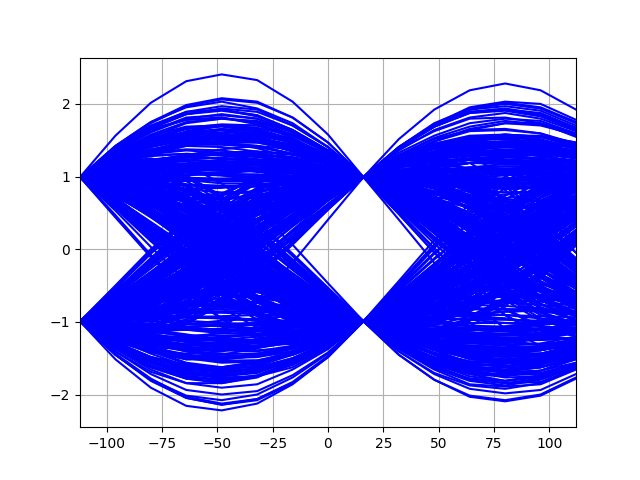
\includegraphics[width=\linewidth]{imagenes_FP/eye_d_filter0q8,7_round.png}
    \end{subfigure}
    \caption{Diagrama de ojo S(8,7) rounded con $\alpha=0$}
    \label{fig:eye_d_filter0q8_7_round}
\end{figure}

\begin{figure}[H]
    \centering

    \begin{subfigure}{0.49\textwidth}
        \centering
        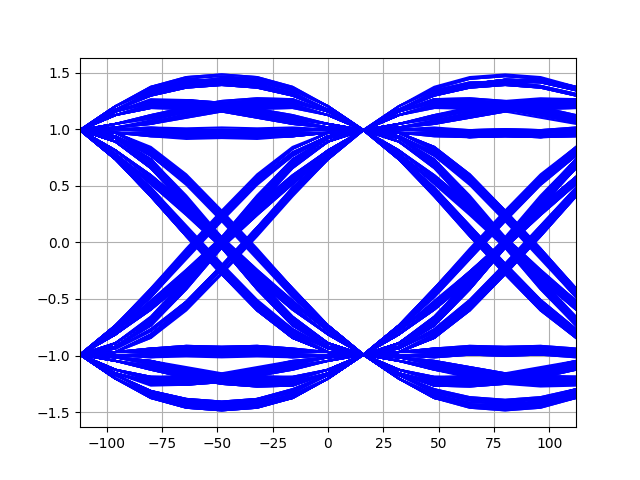
\includegraphics[width=\linewidth]{imagenes_FP/eye_d_filter1i8,7_round.png}
    \end{subfigure}
    \hfill
    \begin{subfigure}{0.49\textwidth}
        \centering
        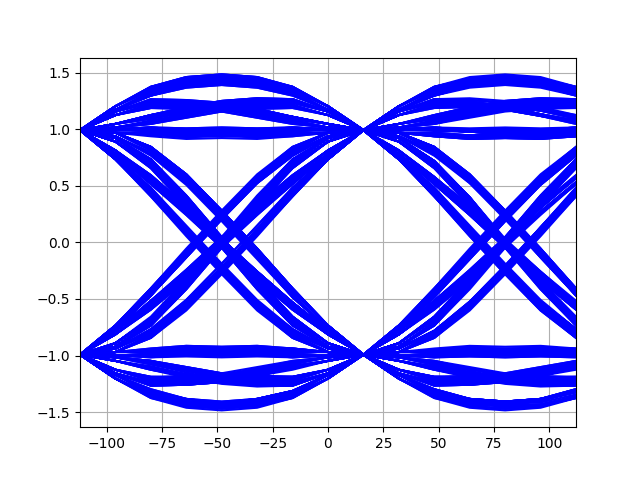
\includegraphics[width=\linewidth]{imagenes_FP/eye_d_filter1q8,7_round.png}
    \end{subfigure}
    \caption{Diagrama de ojo S(8,7) rounded con $\alpha=0.5$}
    \label{fig:eye_d_filter1q8_7_round}
\end{figure}

\begin{figure}[H]
    \centering

    \begin{subfigure}{0.49\textwidth}
        \centering
        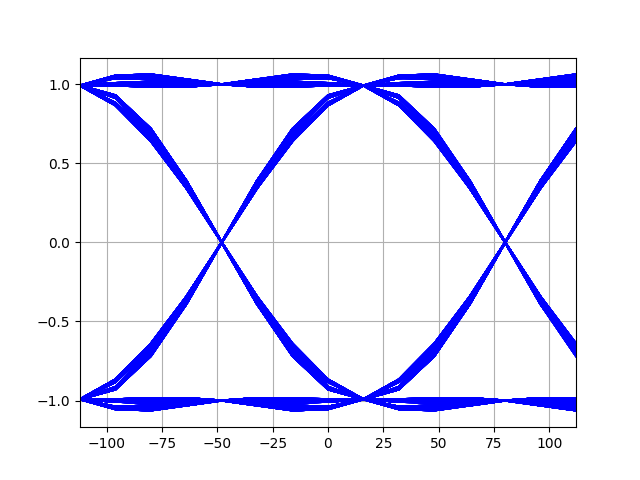
\includegraphics[width=\linewidth]{imagenes_FP/eye_d_filter2i8,7_round.png}
    \end{subfigure}
    \hfill
    \begin{subfigure}{0.49\textwidth}
        \centering
        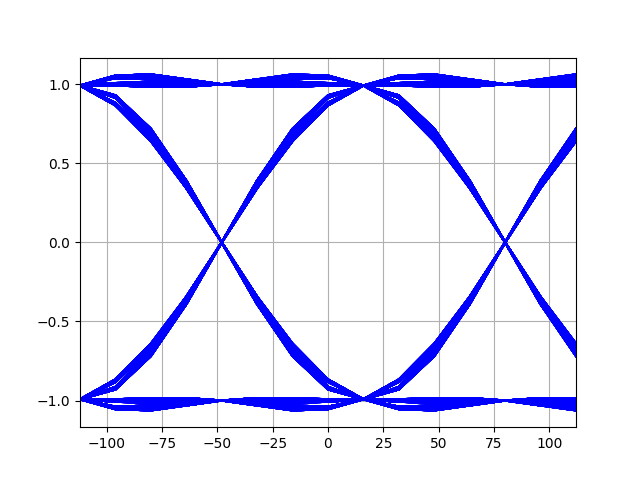
\includegraphics[width=\linewidth]{imagenes_FP/eye_d_filter2q8,7_round.png}
    \end{subfigure}
    \caption{Diagrama de ojo S(8,7) rounded con $\alpha=1$}
    \label{fig:eye_d_filter2q8_7_round}
\end{figure}

\begin{figure}[H]
    \centering

    \begin{subfigure}{0.32\textwidth}
        \centering
        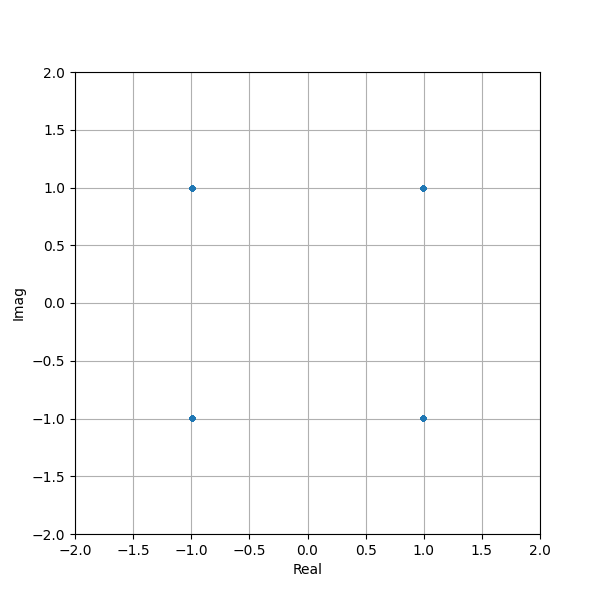
\includegraphics[width=\linewidth]{imagenes_FP/constelation_filters_opt8,7_round.png}
        \caption{$\alpha=0$}
    \end{subfigure}
    \hfill
    \begin{subfigure}{0.32\textwidth}
        \centering
        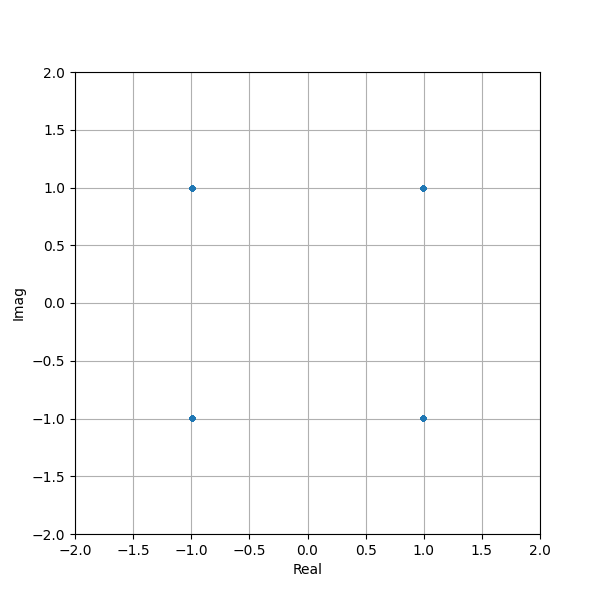
\includegraphics[width=\linewidth]{imagenes_FP/constelation_filters_opt8,7_round.png}
        \caption{$\alpha=0.5$}
    \end{subfigure}
    \hfill
    \begin{subfigure}{0.32\textwidth}
        \centering
        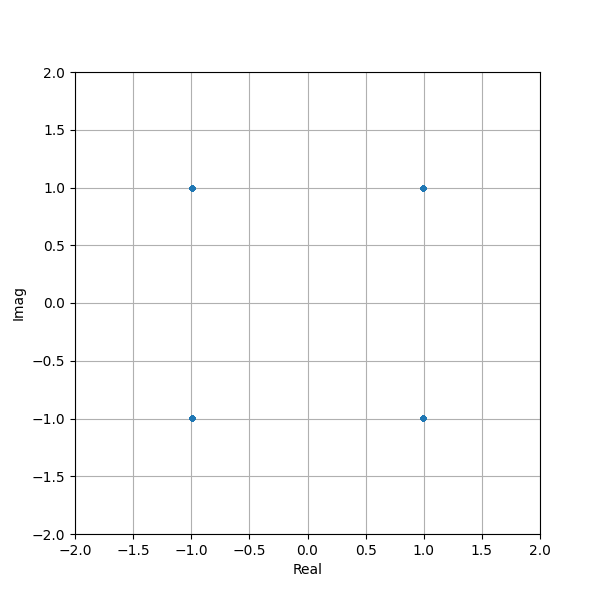
\includegraphics[width=\linewidth]{imagenes_FP/constelation_filters_opt8,7_round.png}
        \caption{$\alpha=1$}
    \end{subfigure}
    \caption{Constelaciones según $\alpha$ para S(8,7) rounded}
    \label{fig:constelations_filters_opt8_7_round}
\end{figure}


\subsection{Cuantización S(3,2)}

Con la cuantización pedida, es imperativo graficar la respuesta al impulso y la respuesta en frecuencia debido a que
la limitada cantidad de bits fraccionarios recortará mucho la resolución
de ambas respuestas, logrando una SNR muy pobre.

\begin{figure}[H]
    \centering

    \begin{subfigure}{0.49\textwidth}
        \centering
        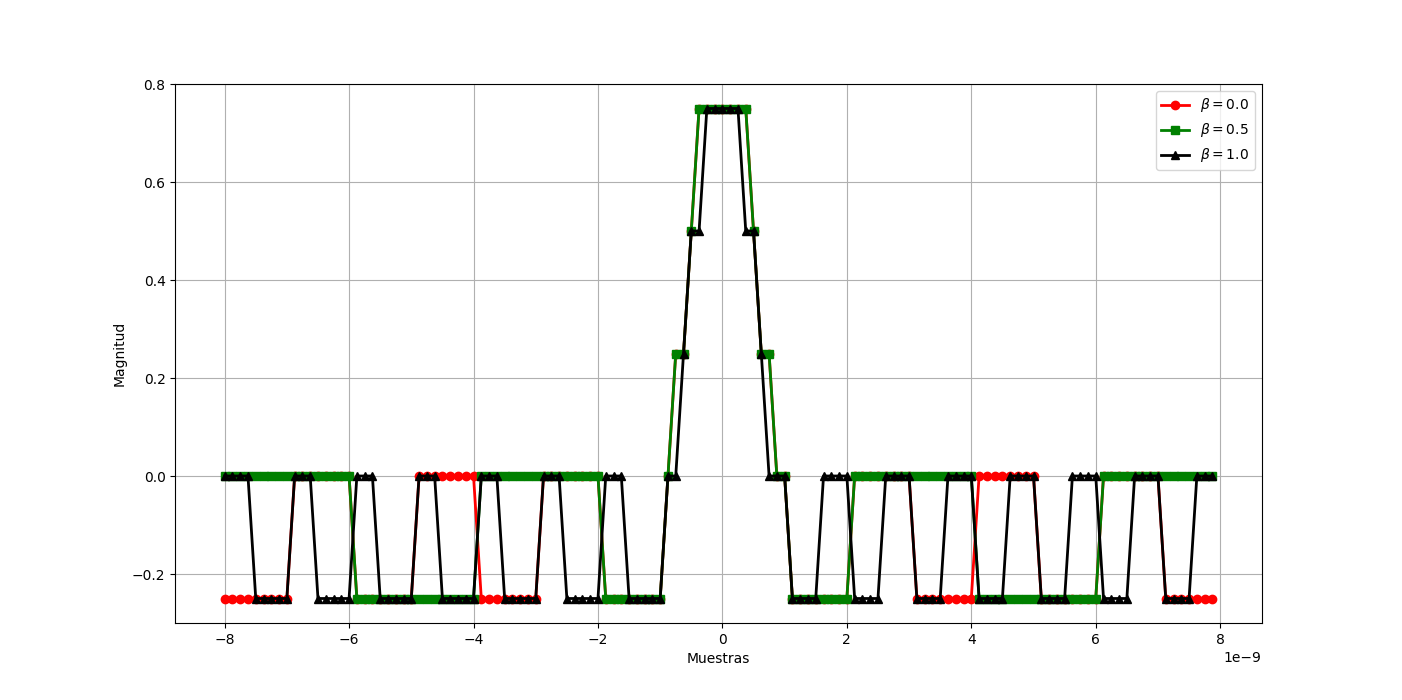
\includegraphics[width=\linewidth]{imagenes_FP/rta_imp_3,2_trunc.png}
        \caption{Respuesta al impulso según $\alpha$}
        \label{fig:rta_imp_3_2_trunc}
    \end{subfigure}
    \hfill
    \begin{subfigure}{0.49\textwidth}
        \centering
        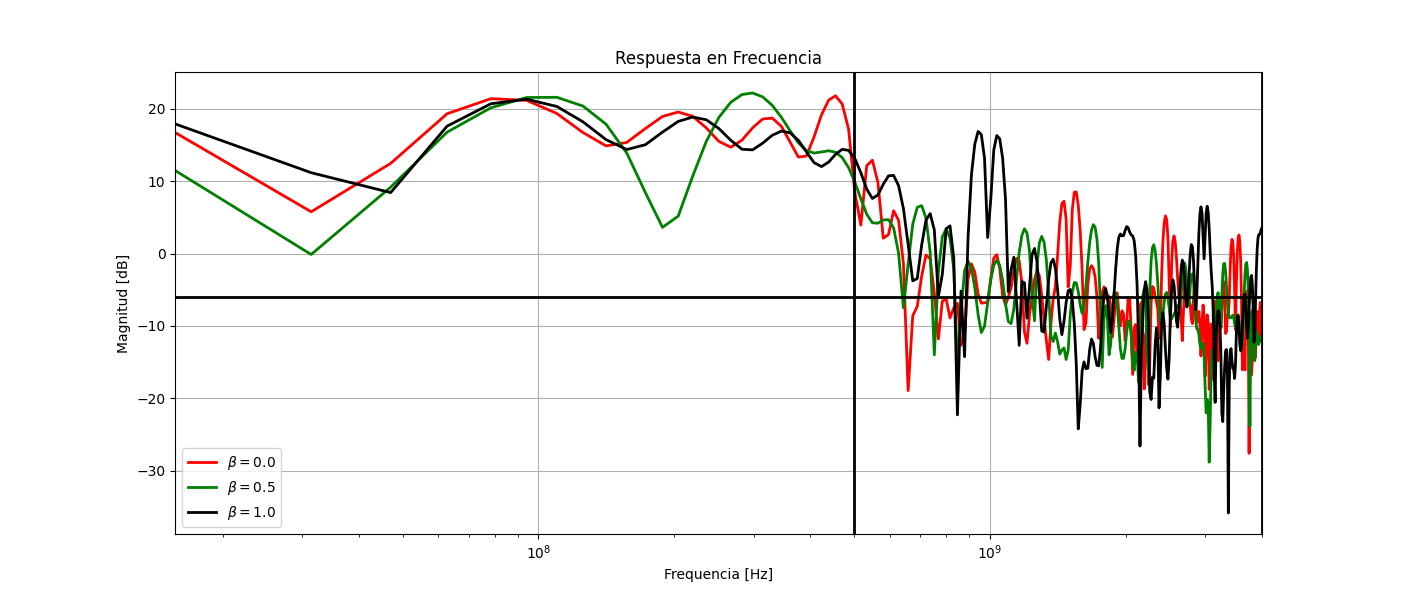
\includegraphics[width=\linewidth]{imagenes_FP/rta_freq_3,2_trunc.png}
        \caption{Respuesta en frecuencia según $\alpha$}
        \label{fig:rta_freq_3_2_trunc}
    \end{subfigure}
    \caption{Respuesta en tiempo y frecuencia S(3,2) truncado}
\end{figure}

\begin{figure}[H]
    \centering

    \begin{subfigure}{0.49\textwidth}
        \centering
        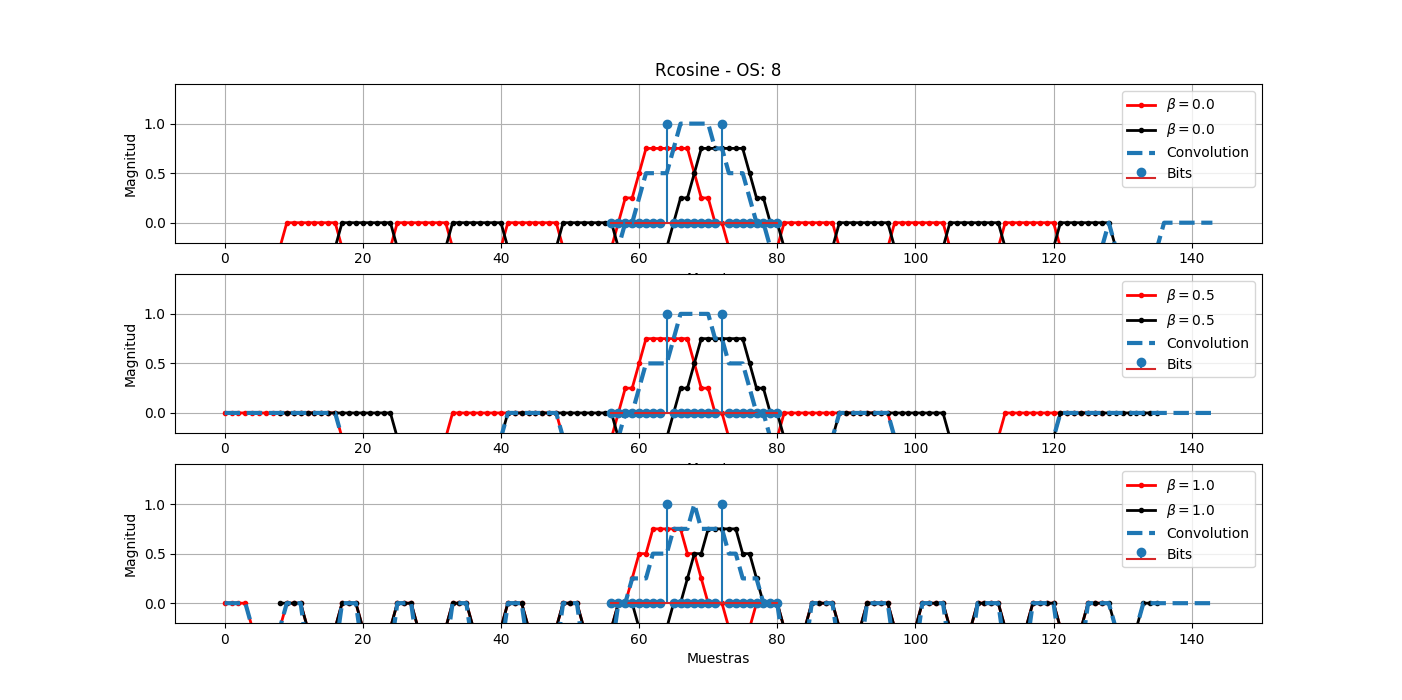
\includegraphics[width=\linewidth]{imagenes_FP/os_effect_3,2_trunc.png}
        \caption{Convolución según $\alpha$}
        \label{fig:os_effect_3_2_trunc}
    \end{subfigure}
    \hfill
    \begin{subfigure}{0.49\textwidth}
        \centering
        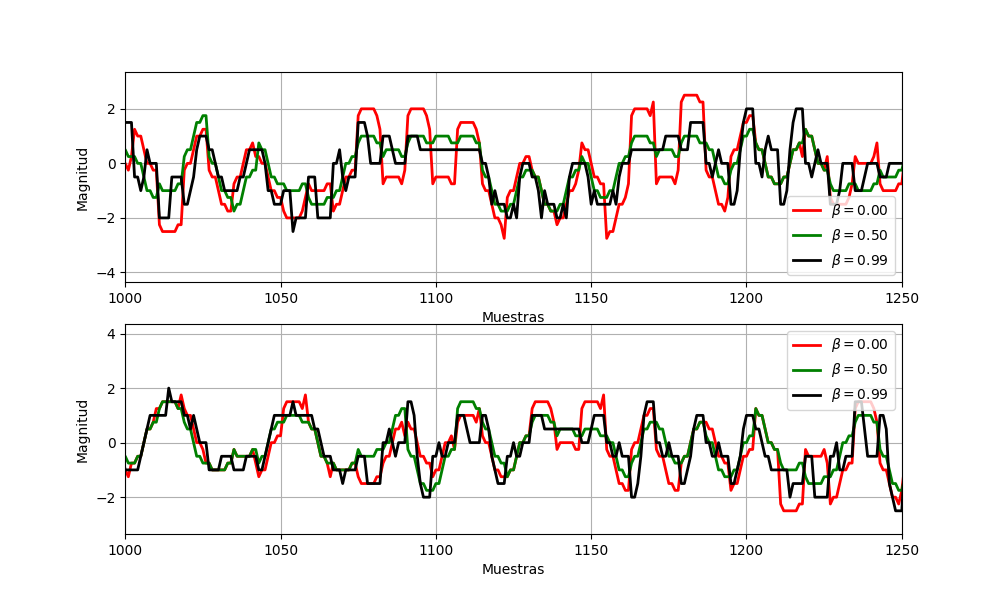
\includegraphics[width=\linewidth]{imagenes_FP/simbols_in_out3,2_trunc.png}
        \caption{Señal transmitida según $\alpha$}
        \label{fig:simbols_in_out3_2_trunc}
    \end{subfigure}
    \caption{Convolución y Transmisión S(3,2) truncado}
\end{figure}

\begin{figure}[H]
    \centering

    \begin{subfigure}{0.49\textwidth}
        \centering
        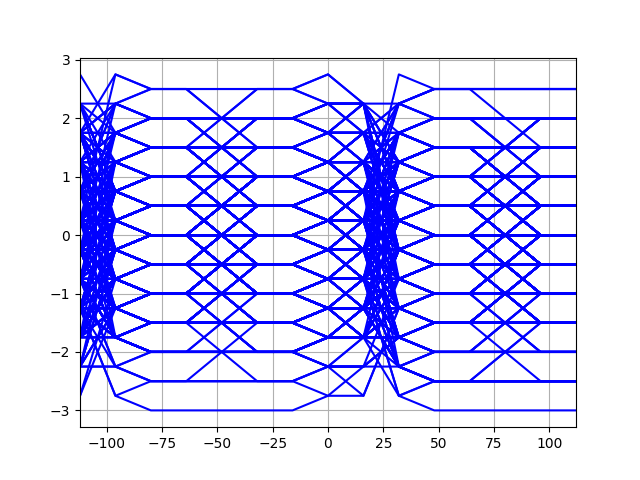
\includegraphics[width=\linewidth]{imagenes_FP/eye_d_filter0i3,2_trunc.png}
    \end{subfigure}
    \hfill
    \begin{subfigure}{0.49\textwidth}
        \centering
        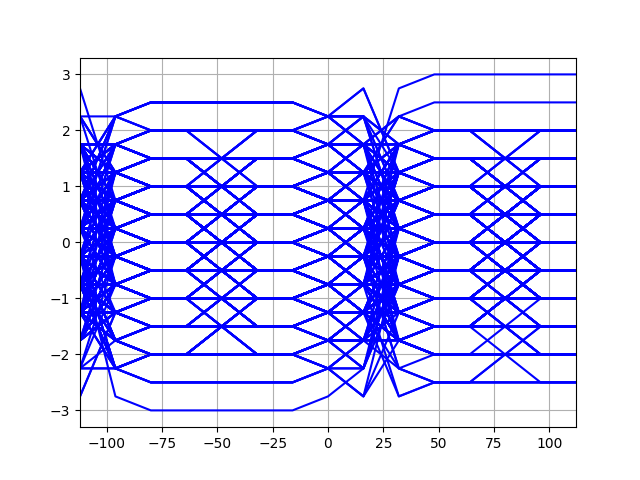
\includegraphics[width=\linewidth]{imagenes_FP/eye_d_filter0q3,2_trunc.png}
    \end{subfigure}
    \caption{Diagrama de ojo S(3,2) truncado con $\alpha=0$}
    \label{fig:eye_d_filter0q3_2_trunc}
\end{figure}

\begin{figure}[H]
    \centering

    \begin{subfigure}{0.49\textwidth}
        \centering
        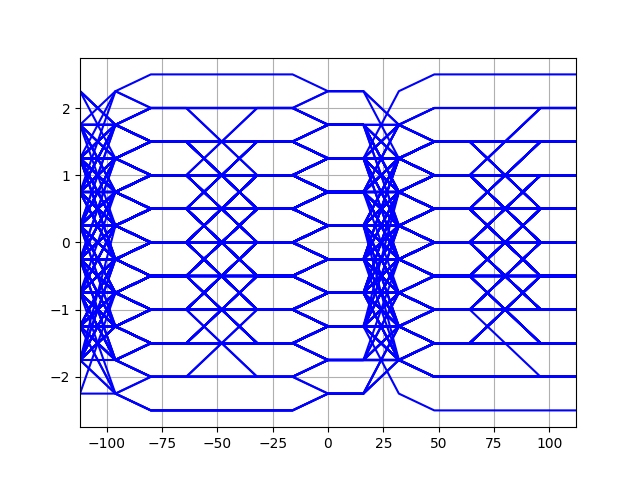
\includegraphics[width=\linewidth]{imagenes_FP/eye_d_filter1i3,2_trunc.png}
    \end{subfigure}
    \hfill
    \begin{subfigure}{0.49\textwidth}
        \centering
        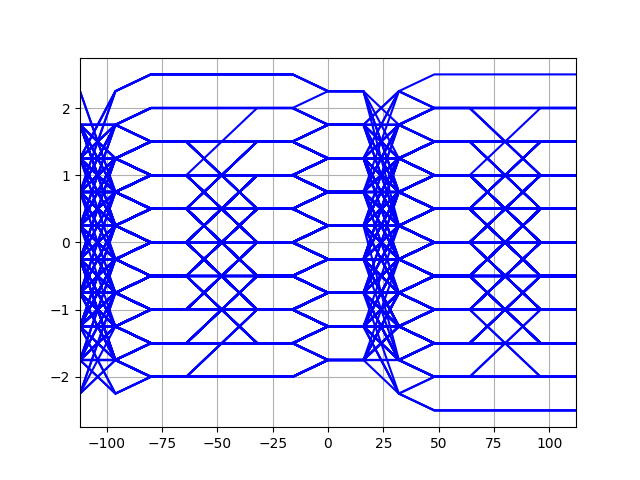
\includegraphics[width=\linewidth]{imagenes_FP/eye_d_filter1q3,2_trunc.png}
    \end{subfigure}
    \caption{Diagrama de ojo S(3,2) truncado con $\alpha=0.5$}
    \label{fig:eye_d_filter1q3_2_trunc}
\end{figure}

\begin{figure}[H]
    \centering

    \begin{subfigure}{0.49\textwidth}
        \centering
        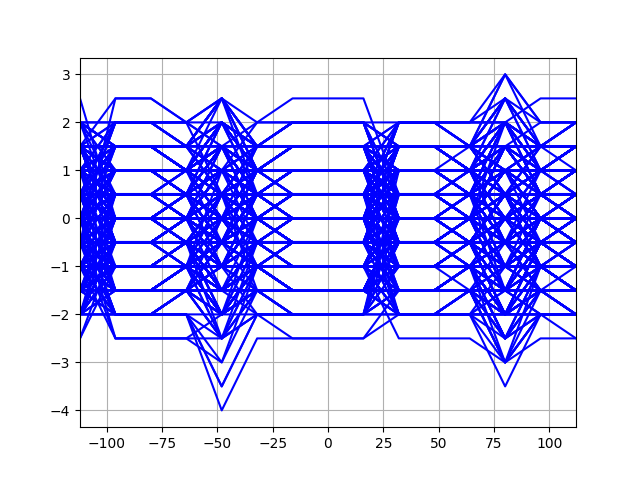
\includegraphics[width=\linewidth]{imagenes_FP/eye_d_filter2i3,2_trunc.png}
    \end{subfigure}
    \hfill
    \begin{subfigure}{0.49\textwidth}
        \centering
        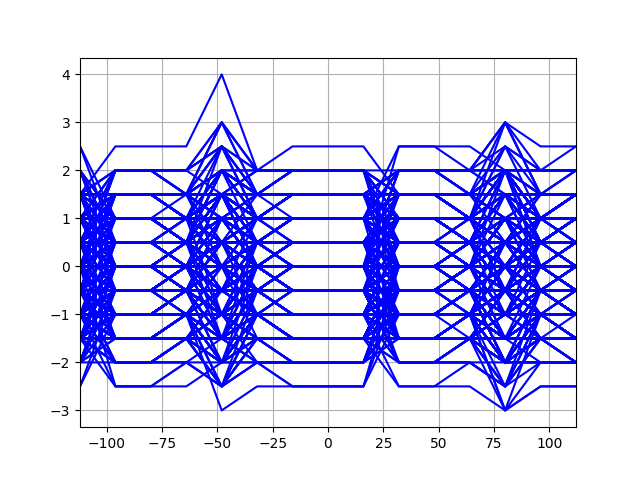
\includegraphics[width=\linewidth]{imagenes_FP/eye_d_filter2q3,2_trunc.png}
    \end{subfigure}
    \caption{Diagrama de ojo S(3,2) truncado con $\alpha=1$}
    \label{fig:eye_d_filter2q3_2_trunc}
\end{figure}

\begin{figure}[H]
    \centering

    \begin{subfigure}{0.32\textwidth}
        \centering
        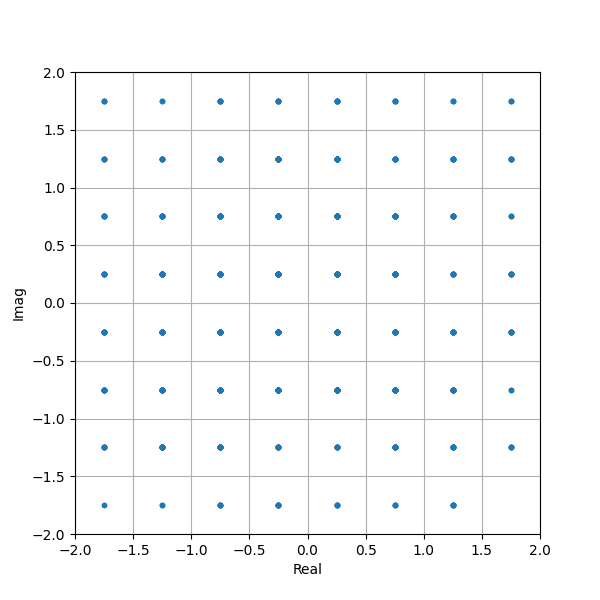
\includegraphics[width=\linewidth]{imagenes_FP/constelation_filter0_opt3,2_trunc.png}
        \caption{$\alpha=0$}
    \end{subfigure}
    \hfill
    \begin{subfigure}{0.32\textwidth}
        \centering
        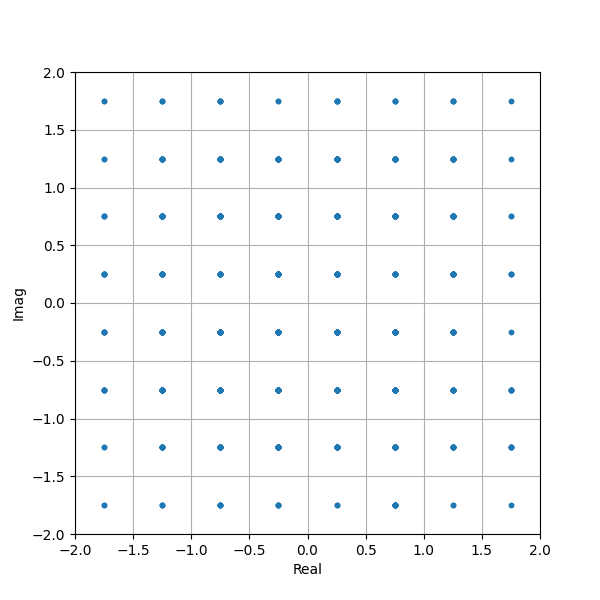
\includegraphics[width=\linewidth]{imagenes_FP/constelation_filter1_opt3,2_trunc.png}
        \caption{$\alpha=0.5$}
    \end{subfigure}
    \hfill
    \begin{subfigure}{0.32\textwidth}
        \centering
        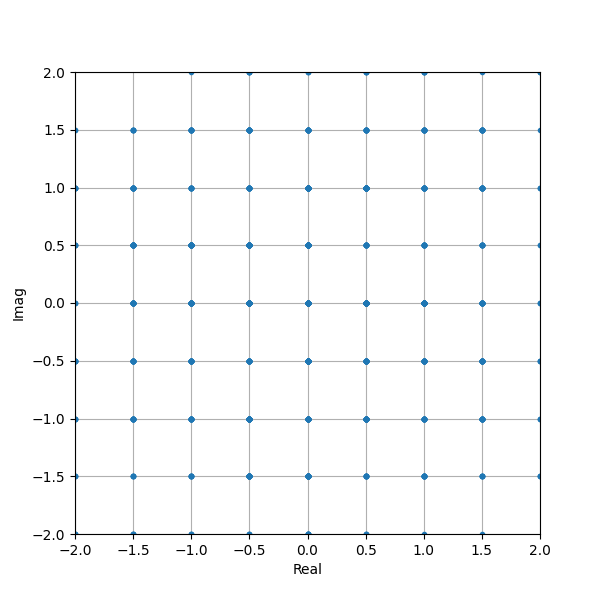
\includegraphics[width=\linewidth]{imagenes_FP/constelation_filter2_opt3,2_trunc.png}
        \caption{$\alpha=1$}
    \end{subfigure}
    \caption{Constelaciones según $\alpha$ para S(3,2) truncado}
    \label{fig:constelations_filters_opt3_2_trunc}
\end{figure}

Ahora, si se utiliza el redondeo se obtienen las siguientes capturas.

\begin{figure}[H]
    \centering

    \begin{subfigure}{0.49\textwidth}
        \centering
        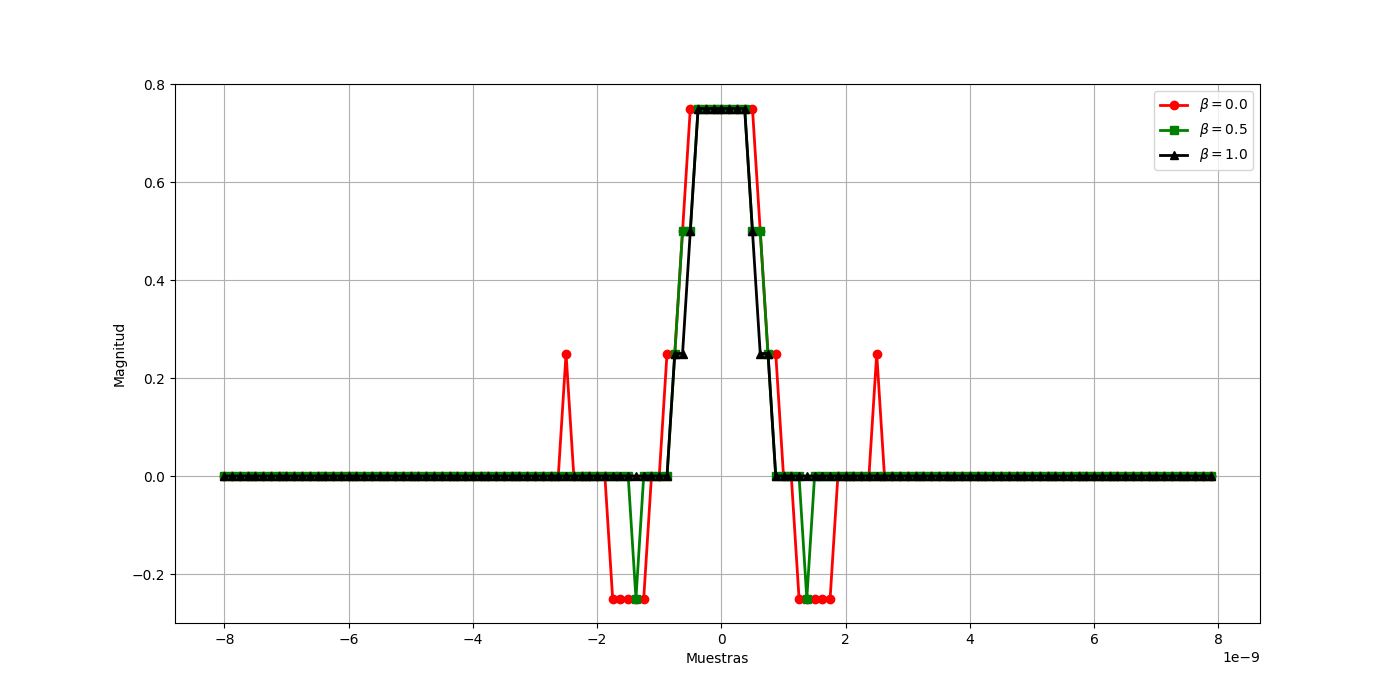
\includegraphics[width=\linewidth]{imagenes_FP/rta_imp_3,2_round.png}
        \caption{Respuesta al impulso según $\alpha$}
        \label{fig:rta_imp_3_2_round}
    \end{subfigure}
    \hfill
    \begin{subfigure}{0.49\textwidth}
        \centering
        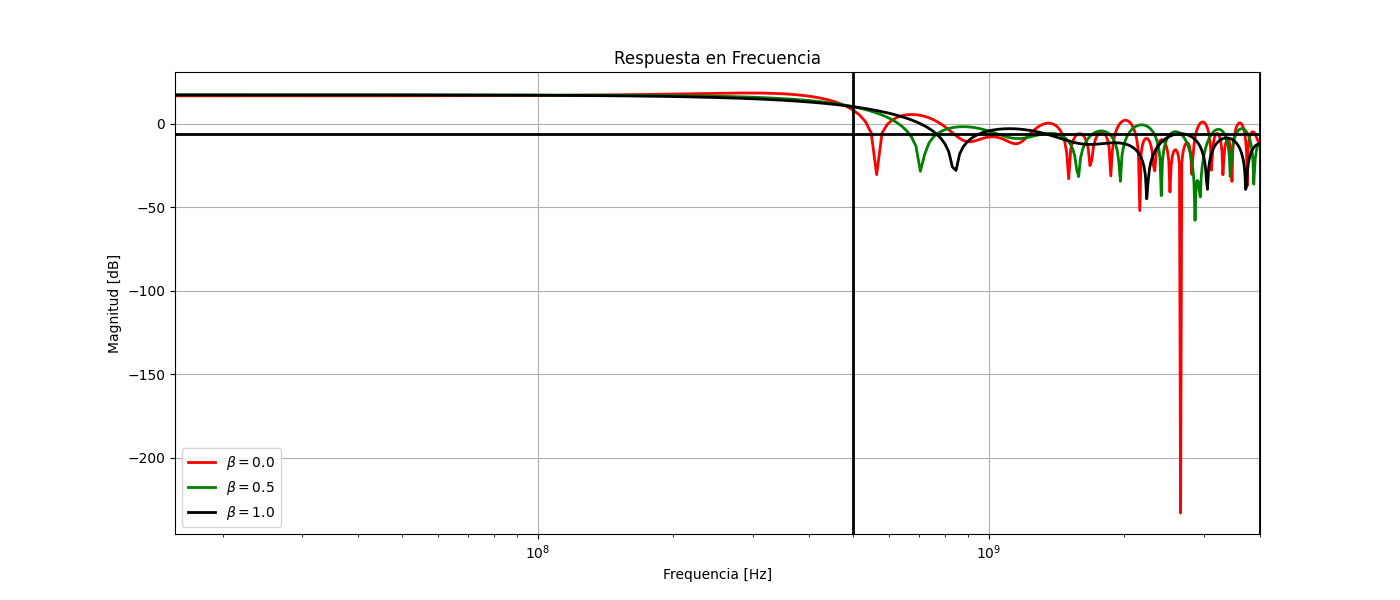
\includegraphics[width=\linewidth]{imagenes_FP/rta_freq_3,2_round.png}
        \caption{Respuesta en frecuencia según $\alpha$}
        \label{fig:rta_freq_3_2_round}
    \end{subfigure}
    \caption{Respuesta en tiempo y frecuencia S(3,2) rounded}
\end{figure}

\begin{figure}[H]
    \centering

    \begin{subfigure}{0.49\textwidth}
        \centering
        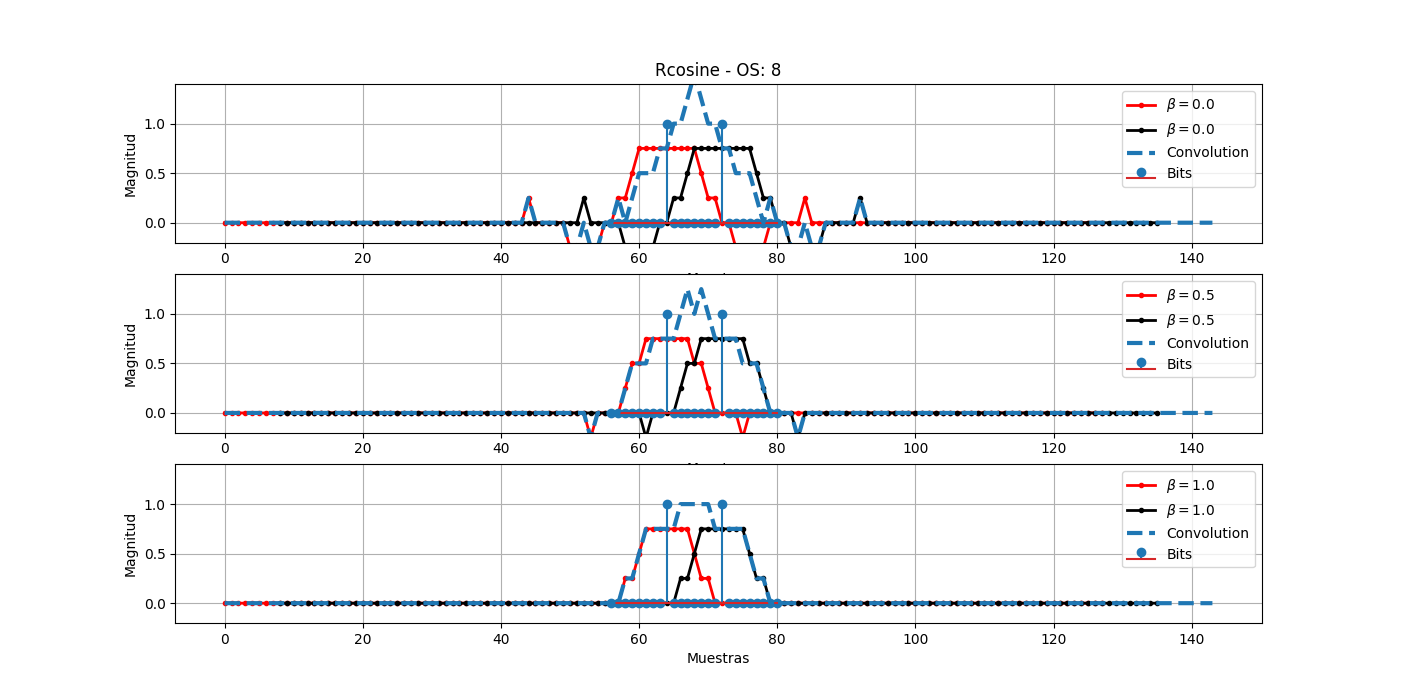
\includegraphics[width=\linewidth]{imagenes_FP/os_effect_3,2_round.png}
        \caption{Convolución según $\alpha$}
        \label{fig:os_effect_3_2_round}
    \end{subfigure}
    \hfill
    \begin{subfigure}{0.49\textwidth}
        \centering
        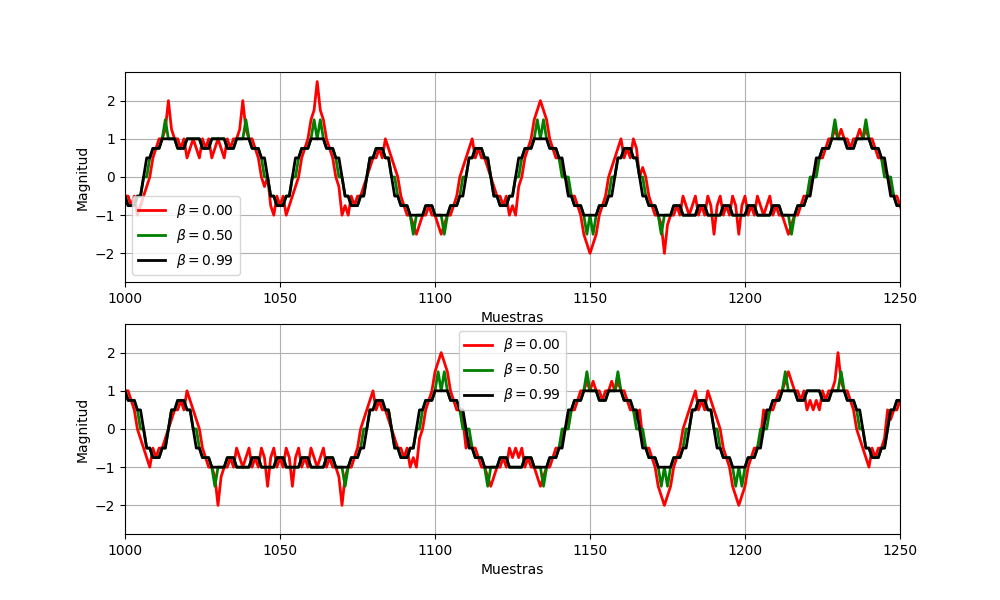
\includegraphics[width=\linewidth]{imagenes_FP/simbols_in_out3,2_round.png}
        \caption{Señal transmitida según $\alpha$}
        \label{fig:simbols_in_out3_2_round}
    \end{subfigure}
    \caption{Convolución y Transmisión S(3,2) rounded}
\end{figure}

\begin{figure}[H]
    \centering

    \begin{subfigure}{0.49\textwidth}
        \centering
        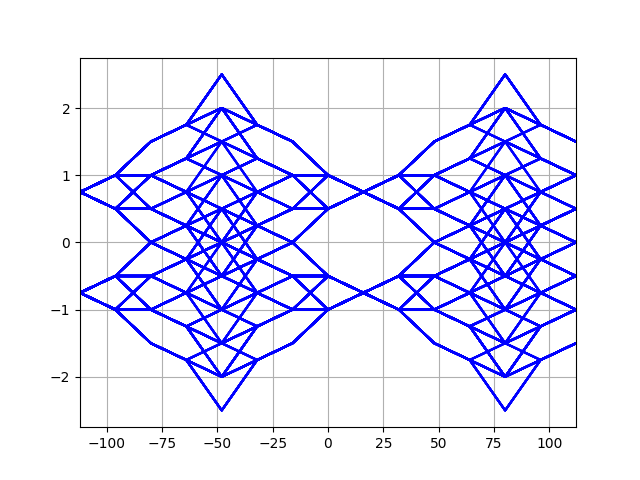
\includegraphics[width=\linewidth]{imagenes_FP/eye_d_filter0i3,2_round.png}
    \end{subfigure}
    \hfill
    \begin{subfigure}{0.49\textwidth}
        \centering
        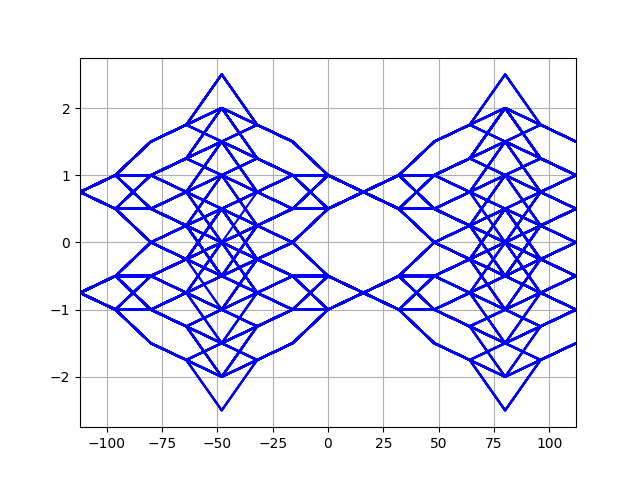
\includegraphics[width=\linewidth]{imagenes_FP/eye_d_filter0q3,2_round.png}
    \end{subfigure}
    \caption{Diagrama de ojo S(3,2) rounded con $\alpha=0$}
    \label{fig:eye_d_filter0q3_2_round}
\end{figure}

\begin{figure}[H]
    \centering

    \begin{subfigure}{0.49\textwidth}
        \centering
        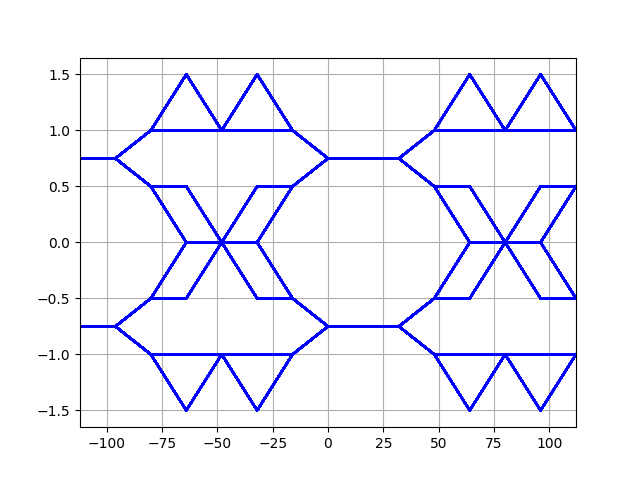
\includegraphics[width=\linewidth]{imagenes_FP/eye_d_filter1i3,2_round.png}
    \end{subfigure}
    \hfill
    \begin{subfigure}{0.49\textwidth}
        \centering
        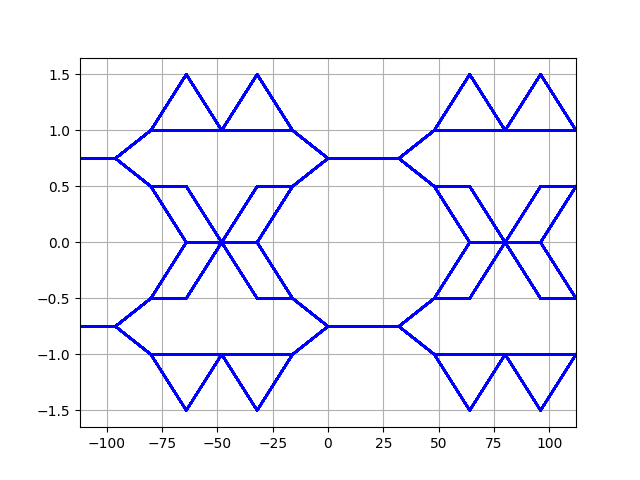
\includegraphics[width=\linewidth]{imagenes_FP/eye_d_filter1q3,2_round.png}
    \end{subfigure}
    \caption{Diagrama de ojo S(3,2) rounded con $\alpha=0.5$}
    \label{fig:eye_d_filter1q3_2_round}
\end{figure}

\begin{figure}[H]
    \centering

    \begin{subfigure}{0.49\textwidth}
        \centering
        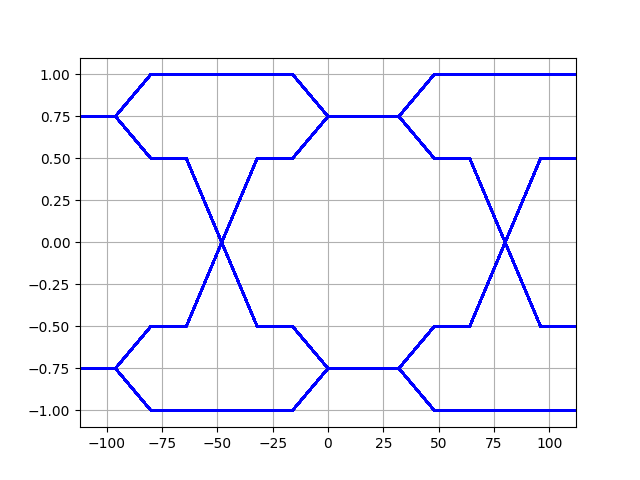
\includegraphics[width=\linewidth]{imagenes_FP/eye_d_filter2i3,2_round.png}
    \end{subfigure}
    \hfill
    \begin{subfigure}{0.49\textwidth}
        \centering
        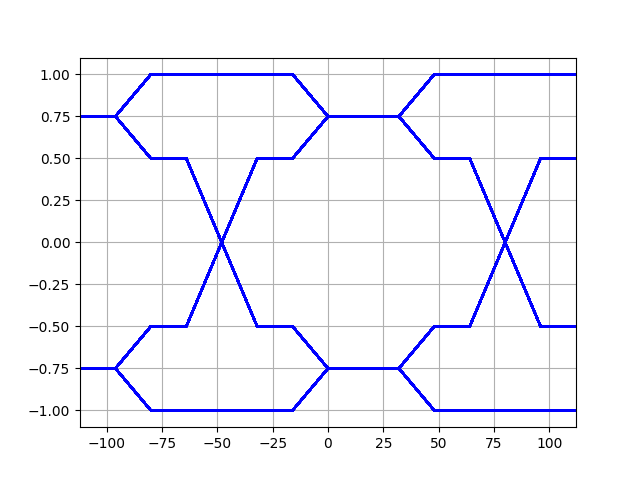
\includegraphics[width=\linewidth]{imagenes_FP/eye_d_filter2q3,2_round.png}
    \end{subfigure}
    \caption{Diagrama de ojo S(3,2) rounded con $\alpha=1$}
    \label{fig:eye_d_filter2q3_2_round}
\end{figure}

\begin{figure}[H]
    \centering

    \begin{subfigure}{0.32\textwidth}
        \centering
        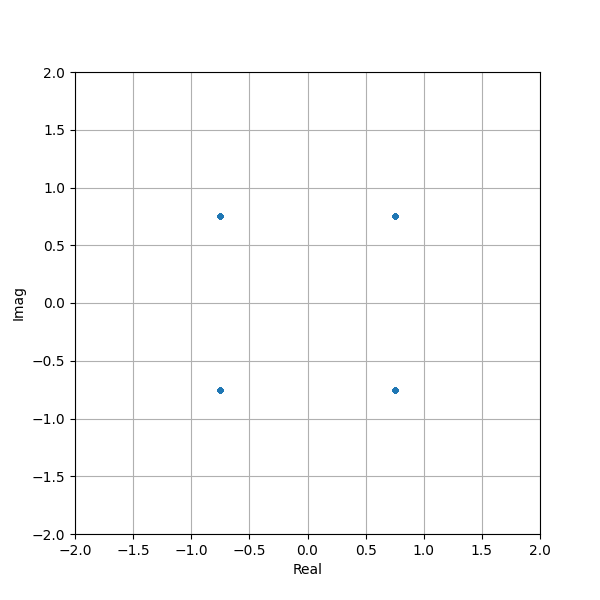
\includegraphics[width=\linewidth]{imagenes_FP/constelation_filters_opt3,2_round.png}
        \caption{$\alpha=0$}
    \end{subfigure}
    \hfill
    \begin{subfigure}{0.32\textwidth}
        \centering
        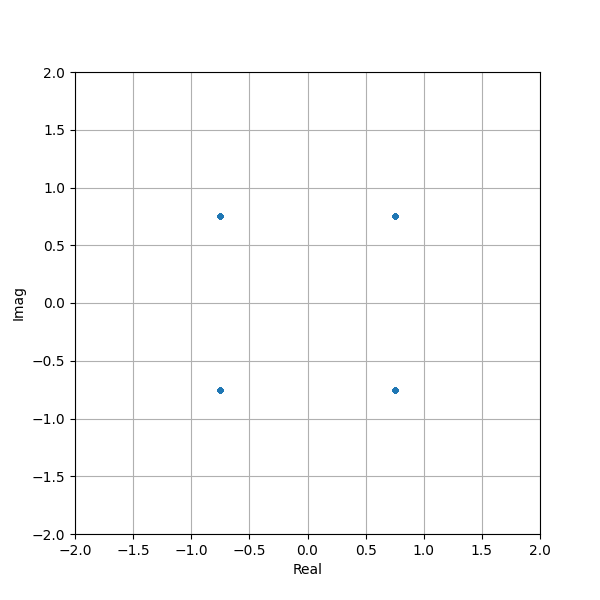
\includegraphics[width=\linewidth]{imagenes_FP/constelation_filters_opt3,2_round.png}
        \caption{$\alpha=0.5$}
    \end{subfigure}
    \hfill
    \begin{subfigure}{0.32\textwidth}
        \centering
        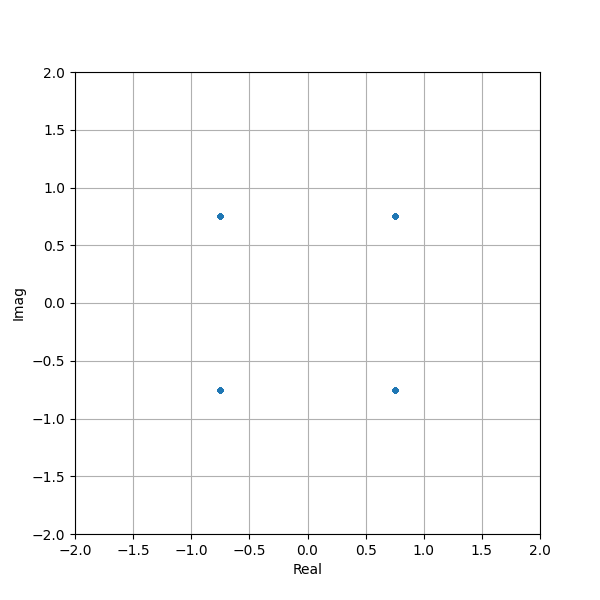
\includegraphics[width=\linewidth]{imagenes_FP/constelation_filters_opt3,2_round.png}
        \caption{$\alpha=1$}
    \end{subfigure}
    \caption{Constelaciones según $\alpha$ para S(3,2) rounded}
    \label{fig:constelations_filters_opt3_2_round}
\end{figure}

\subsection{Cuantización S(6,4)}

 Para la última cuantización solicitada, se analizarán todos los gráficos nuevamente, debido a que con la 
 misma se llegará a una conclusión importante.

 \begin{figure}[H]
    \centering

    \begin{subfigure}{0.49\textwidth}
        \centering
        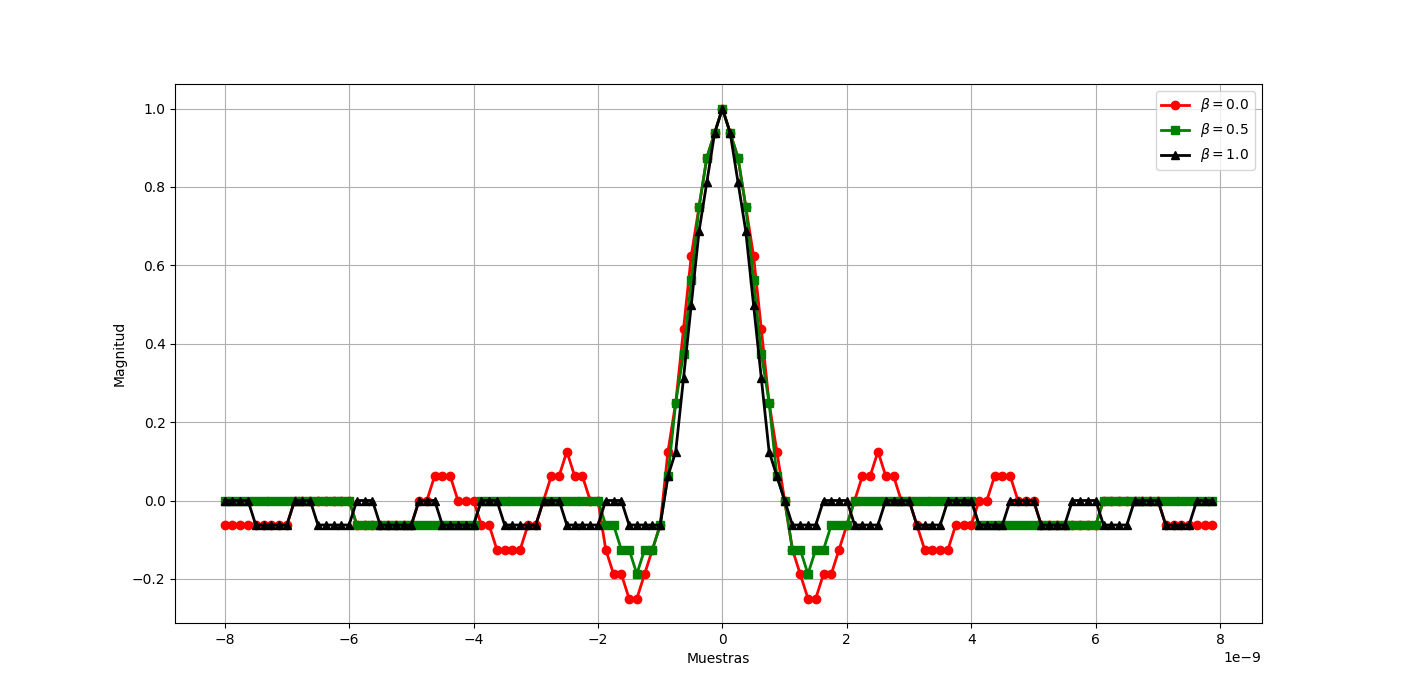
\includegraphics[width=\linewidth]{imagenes_FP/rta_imp_6,4_trunc.png}
        \caption{Respuesta al impulso según $\alpha$}
        \label{fig:rta_imp_6_4_trunc}
    \end{subfigure}
    \hfill
    \begin{subfigure}{0.49\textwidth}
        \centering
        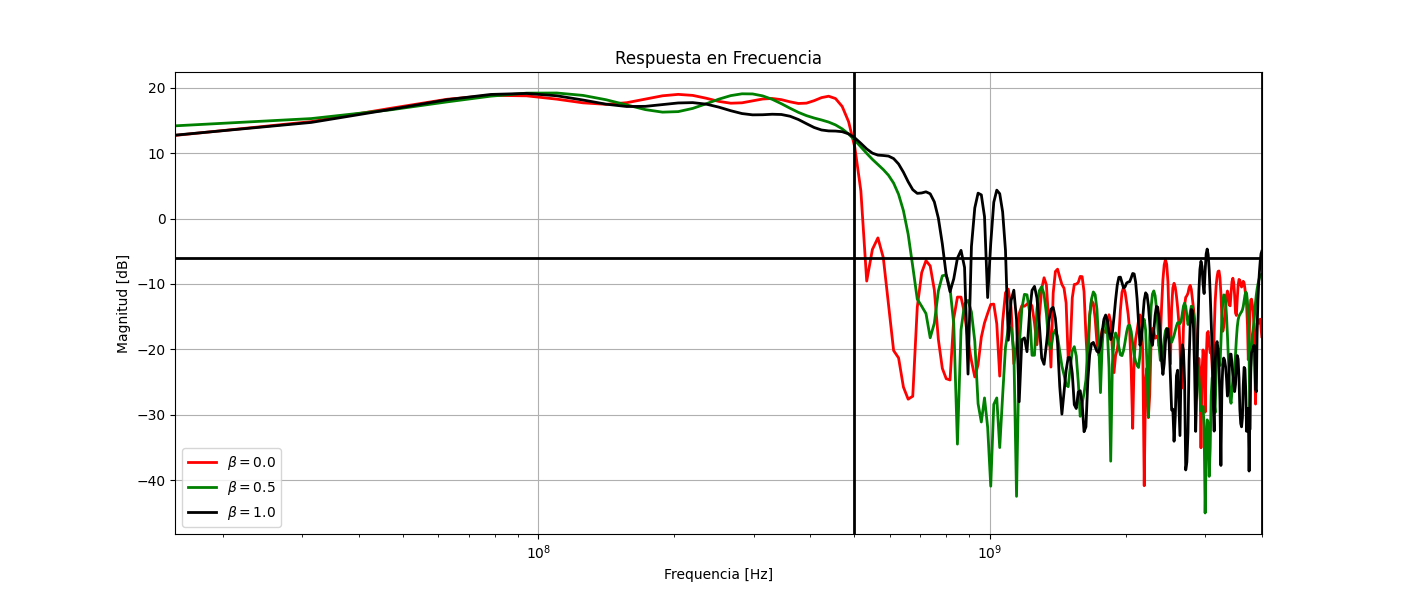
\includegraphics[width=\linewidth]{imagenes_FP/rta_freq_6,4_trunc.png}
        \caption{Respuesta en frecuencia según $\alpha$}
        \label{fig:rta_freq_6_4_trunc}
    \end{subfigure}
    \caption{Respuesta en tiempo y frecuencia S(6,4) truncado}
\end{figure}

\begin{figure}[H]
    \centering

    \begin{subfigure}{0.49\textwidth}
        \centering
        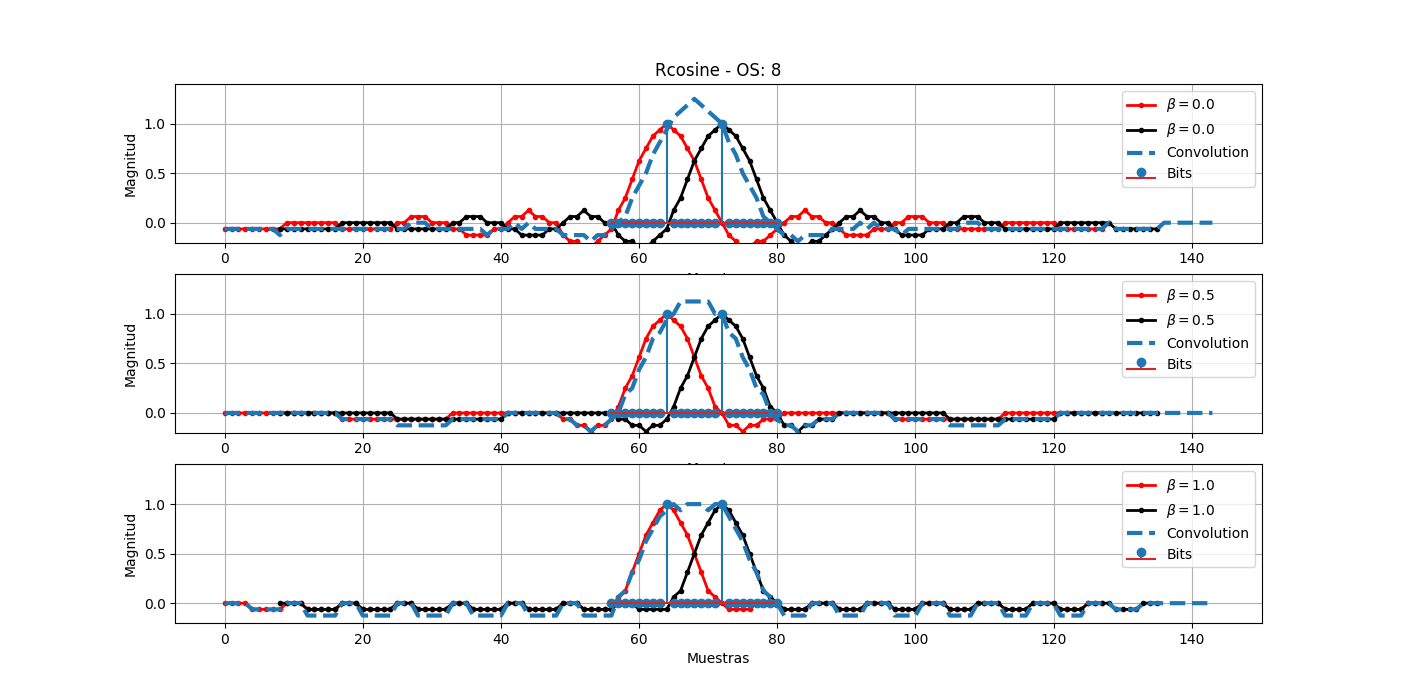
\includegraphics[width=\linewidth]{imagenes_FP/os_effect_6,4_trunc.png}
        \caption{Convolución según $\alpha$}
        \label{fig:os_effect_6_4_trunc}
    \end{subfigure}
    \hfill
    \begin{subfigure}{0.49\textwidth}
        \centering
        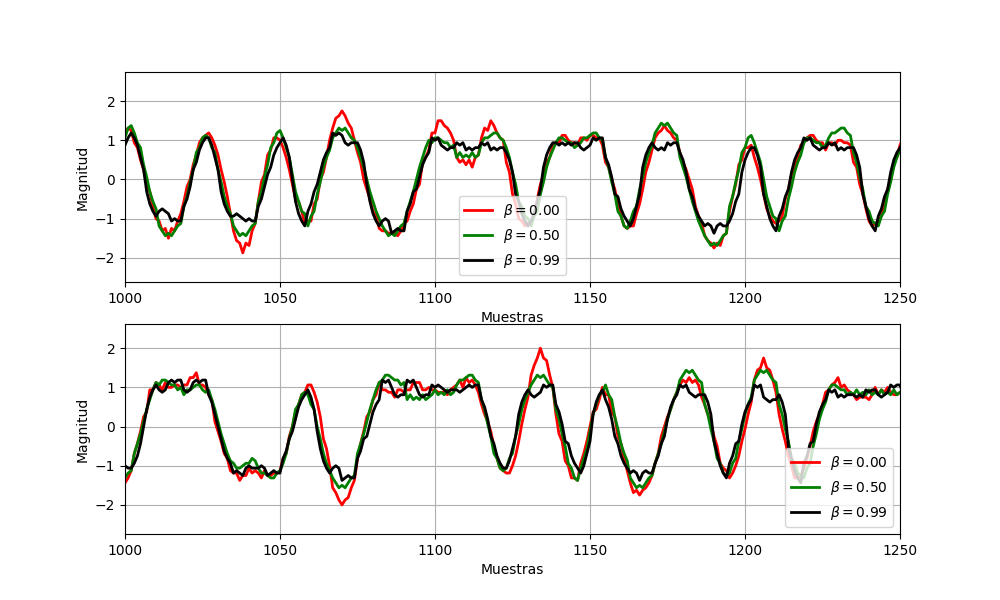
\includegraphics[width=\linewidth]{imagenes_FP/simbols_in_out6,4_trunc.png}
        \caption{Señal transmitida según $\alpha$}
        \label{fig:simbols_in_out6_4_trunc}
    \end{subfigure}
    \caption{Convolución y Transmisión S(6,4) truncado}
\end{figure}

\begin{figure}[H]
    \centering

    \begin{subfigure}{0.49\textwidth}
        \centering
        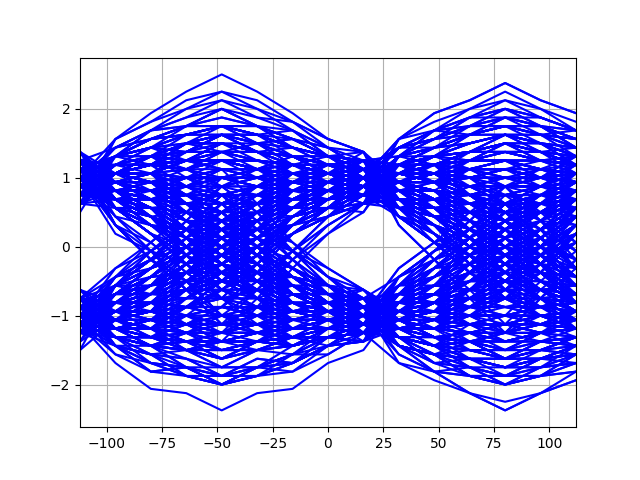
\includegraphics[width=\linewidth]{imagenes_FP/eye_d_filter0i6,4_trunc.png}
    \end{subfigure}
    \hfill
    \begin{subfigure}{0.49\textwidth}
        \centering
        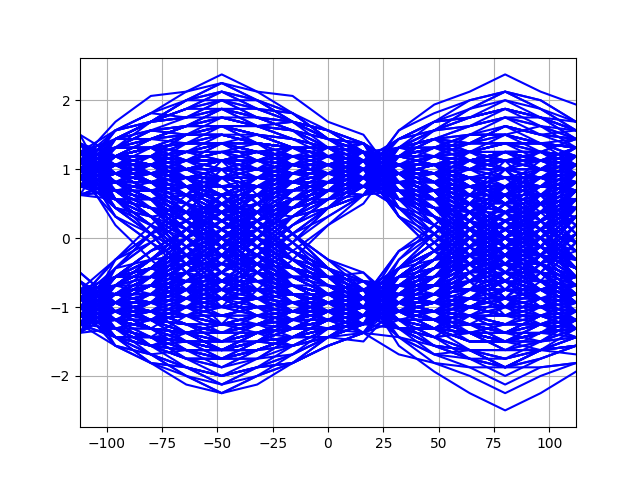
\includegraphics[width=\linewidth]{imagenes_FP/eye_d_filter0q6,4_trunc.png}
    \end{subfigure}
    \label{fig:eye_d_filter0q6_4_trunc}
    \caption{Diagrama de ojo S(6,4) truncado con $\alpha=0$}
\end{figure}

\begin{figure}[H]
    \centering

    \begin{subfigure}{0.49\textwidth}
        \centering
        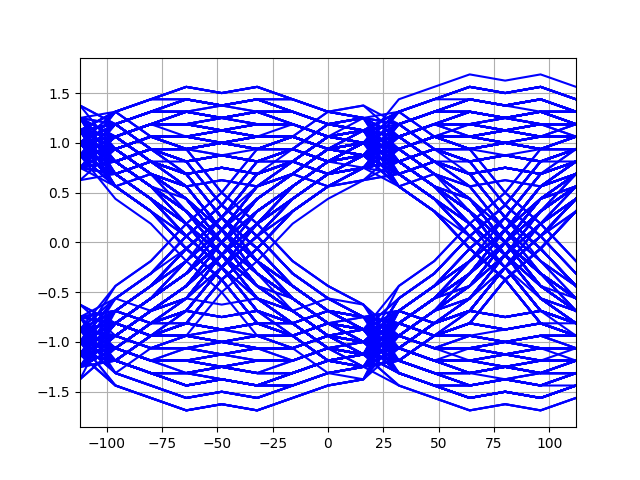
\includegraphics[width=\linewidth]{imagenes_FP/eye_d_filter1i6,4_trunc.png}
    \end{subfigure}
    \hfill
    \begin{subfigure}{0.49\textwidth}
        \centering
        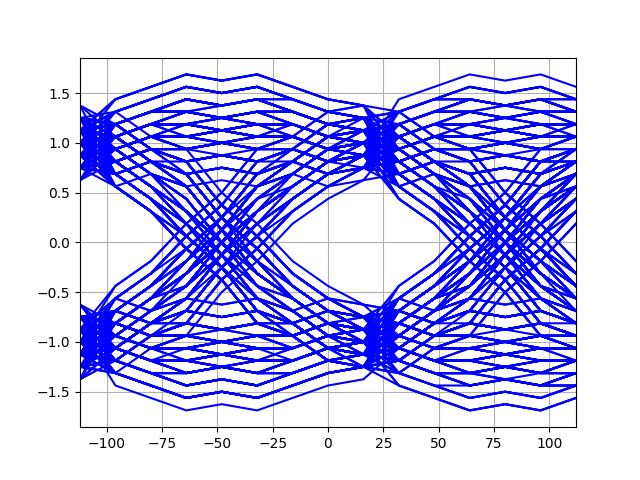
\includegraphics[width=\linewidth]{imagenes_FP/eye_d_filter1q6,4_trunc.png}
    \end{subfigure}
    \caption{Diagrama de ojo S(6,4) truncado con $\alpha=0.5$}
    \label{fig:eye_d_filter1q6_4_trunc}
\end{figure}

\begin{figure}[H]
    \centering

    \begin{subfigure}{0.49\textwidth}
        \centering
        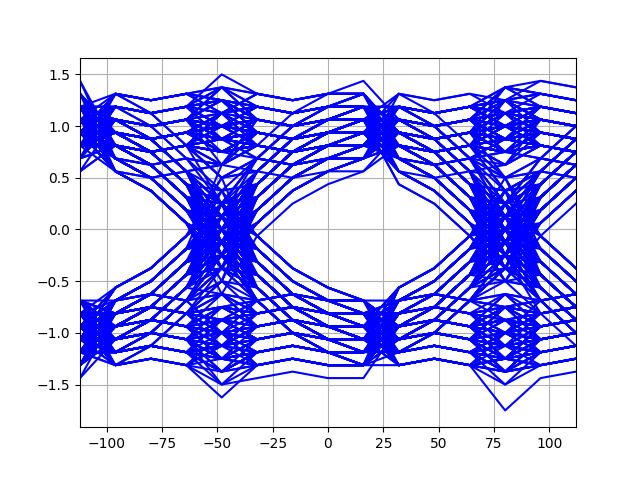
\includegraphics[width=\linewidth]{imagenes_FP/eye_d_filter2i6,4_trunc.png}
    \end{subfigure}
    \hfill
    \begin{subfigure}{0.49\textwidth}
        \centering
        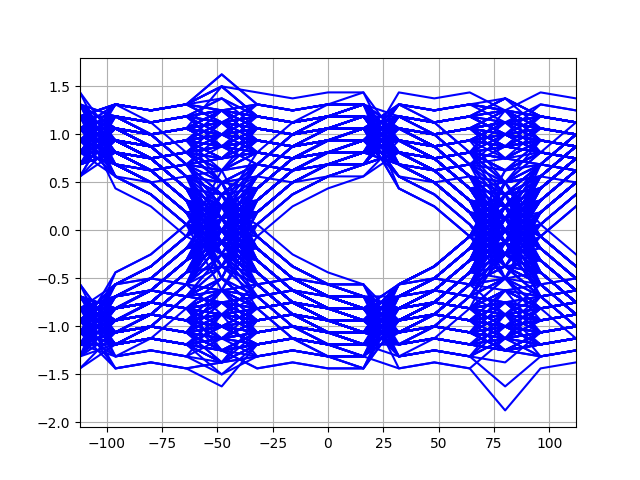
\includegraphics[width=\linewidth]{imagenes_FP/eye_d_filter2q6,4_trunc.png}
    \end{subfigure}
    \caption{Diagrama de ojo S(6,4) truncado con $\alpha=1$}
    \label{fig:eye_d_filter2q6_4_trunc}
\end{figure}

\begin{figure}[H]
    \centering

    \begin{subfigure}{0.32\textwidth}
        \centering
        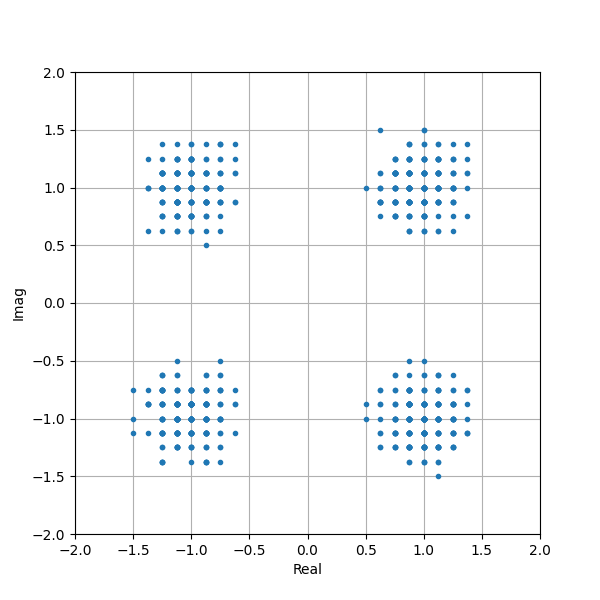
\includegraphics[width=\linewidth]{imagenes_FP/constelation_filter0_opt6,4_trunc.png}
        \caption{$\alpha=0$}
    \end{subfigure}
    \hfill
    \begin{subfigure}{0.32\textwidth}
        \centering
        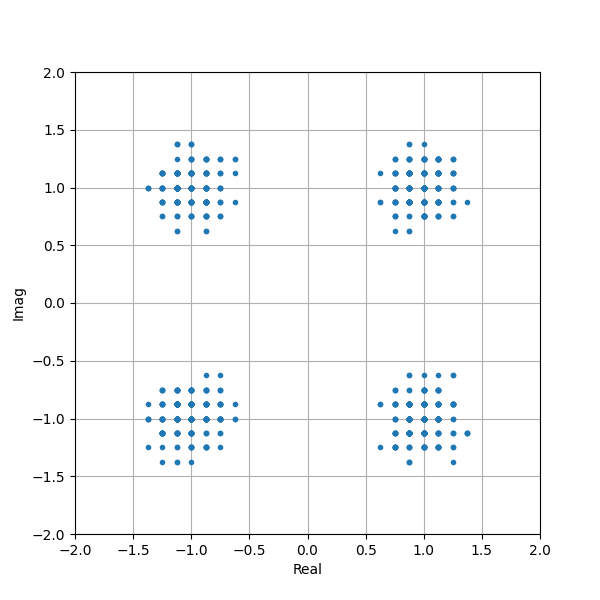
\includegraphics[width=\linewidth]{imagenes_FP/constelation_filter1_opt6,4_trunc.png}
        \caption{$\alpha=0.5$}
    \end{subfigure}
    \hfill
    \begin{subfigure}{0.32\textwidth}
        \centering
        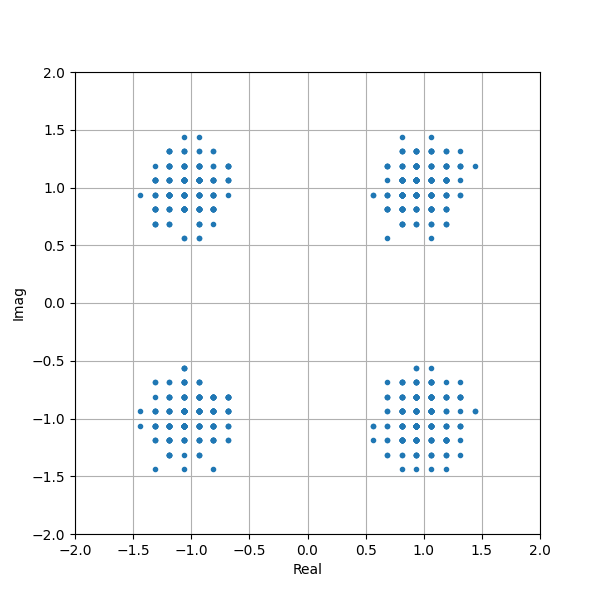
\includegraphics[width=\linewidth]{imagenes_FP/constelation_filter2_opt6,4_trunc.png}
        \caption{$\alpha=1$}
    \end{subfigure}
    \caption{Constelaciones según $\alpha$ para S(6,4) truncado}
    \label{fig:constelations_filters_opt6_4_trunc}
\end{figure}

Ahora, si se utiliza el redondeo se obtienen las siguientes capturas.

\begin{figure}[H]
    \centering

    \begin{subfigure}{0.49\textwidth}
        \centering
        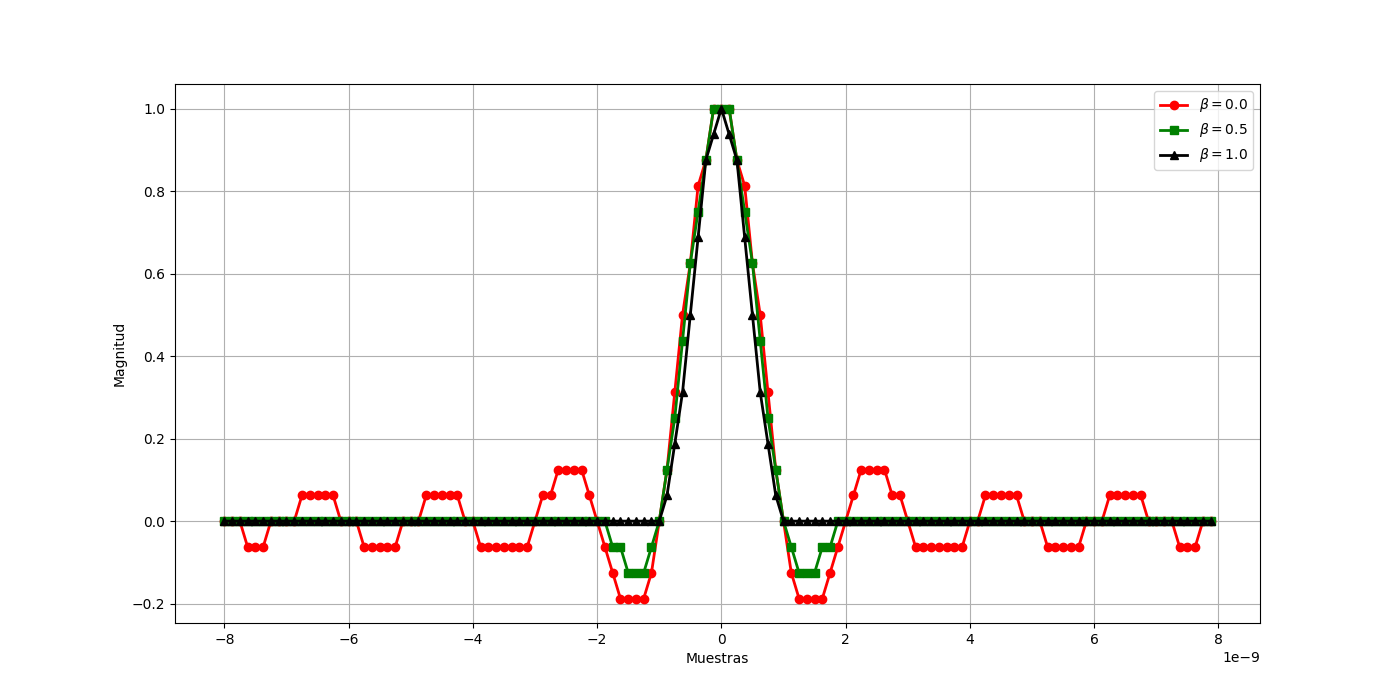
\includegraphics[width=\linewidth]{imagenes_FP/rta_imp_6,4_round.png}
        \caption{Respuesta al impulso según $\alpha$}
        \label{fig:rta_imp_6_4_round}
    \end{subfigure}
    \hfill
    \begin{subfigure}{0.49\textwidth}
        \centering
        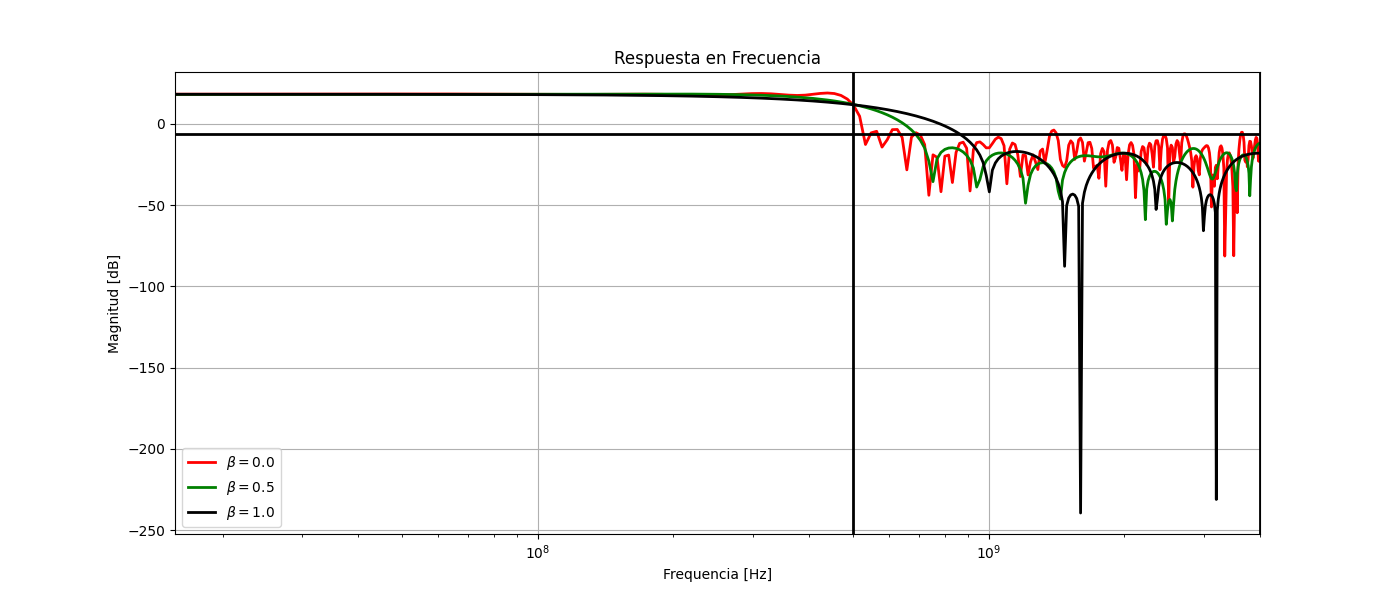
\includegraphics[width=\linewidth]{imagenes_FP/rta_freq_6,4_round.png}
        \caption{Respuesta en frecuencia según $\alpha$}
        \label{fig:rta_freq_6_4_round}
    \end{subfigure}
    \caption{Respuesta en tiempo y frecuencia S(6,4) rounded}
\end{figure}

\begin{figure}[H]
    \centering

    \begin{subfigure}{0.49\textwidth}
        \centering
        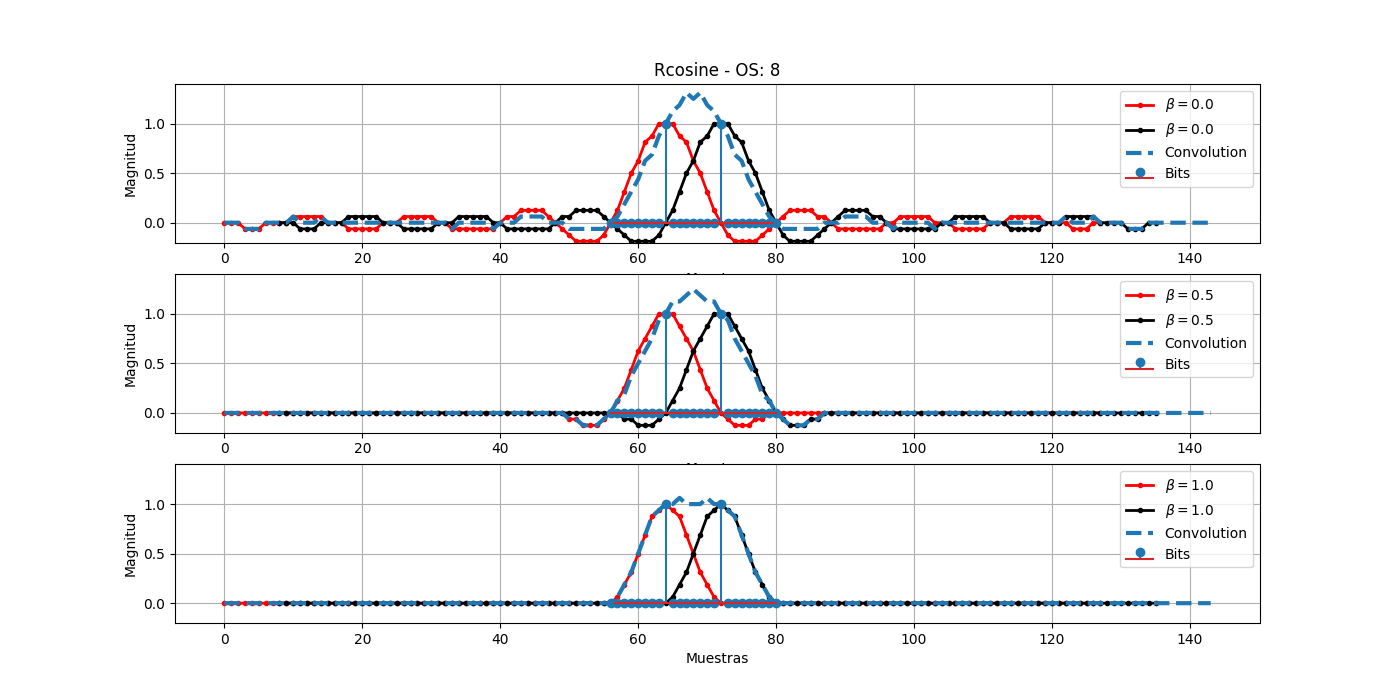
\includegraphics[width=\linewidth]{imagenes_FP/os_effect_6,4_round.png}
        \caption{Convolución según $\alpha$}
        \label{fig:os_effect_6_4_round}
    \end{subfigure}
    \hfill
    \begin{subfigure}{0.49\textwidth}
        \centering
        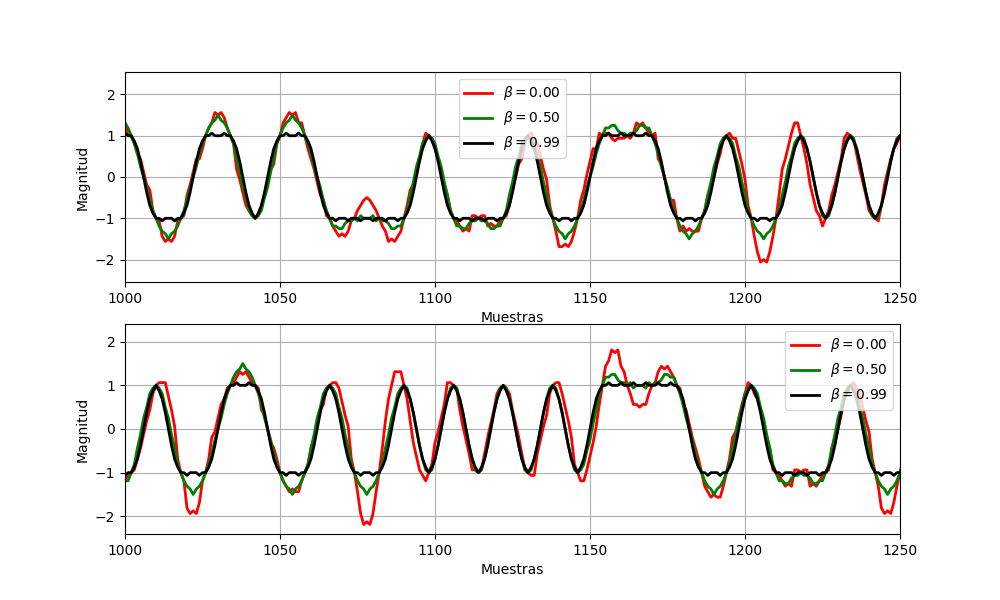
\includegraphics[width=\linewidth]{imagenes_FP/simbols_in_out6,4_round.png}
        \caption{Señal transmitida según $\alpha$}
        \label{fig:simbols_in_out6_4_round}
    \end{subfigure}
    \caption{Convolución y Transmisión S(6,4) rounded}
\end{figure}

\begin{figure}[H]
    \centering

    \begin{subfigure}{0.49\textwidth}
        \centering
        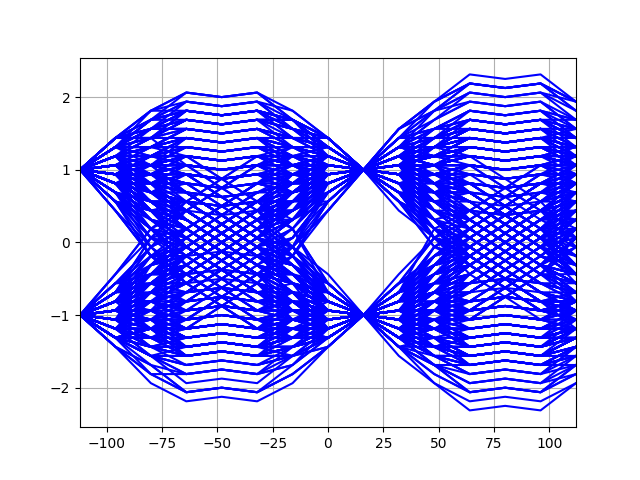
\includegraphics[width=\linewidth]{imagenes_FP/eye_d_filter0i6,4_round.png}
    \end{subfigure}
    \hfill
    \begin{subfigure}{0.49\textwidth}
        \centering
        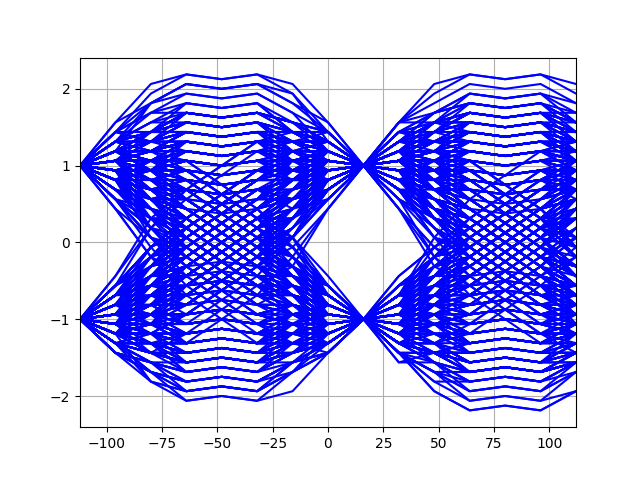
\includegraphics[width=\linewidth]{imagenes_FP/eye_d_filter0q6,4_round.png}
    \end{subfigure}
    \caption{Diagrama de ojo S(6,4) rounded con $\alpha=0$}
    \label{fig:eye_d_filter0q6_4_round}
\end{figure}

\begin{figure}[H]
    \centering

    \begin{subfigure}{0.49\textwidth}
        \centering
        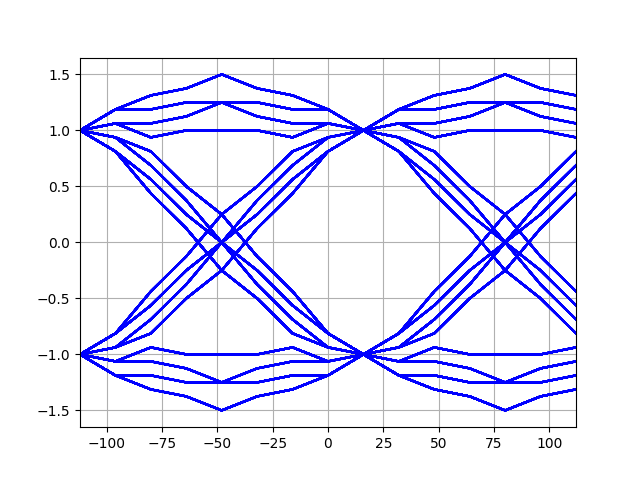
\includegraphics[width=\linewidth]{imagenes_FP/eye_d_filter1i6,4_round.png}
    \end{subfigure}
    \hfill
    \begin{subfigure}{0.49\textwidth}
        \centering
        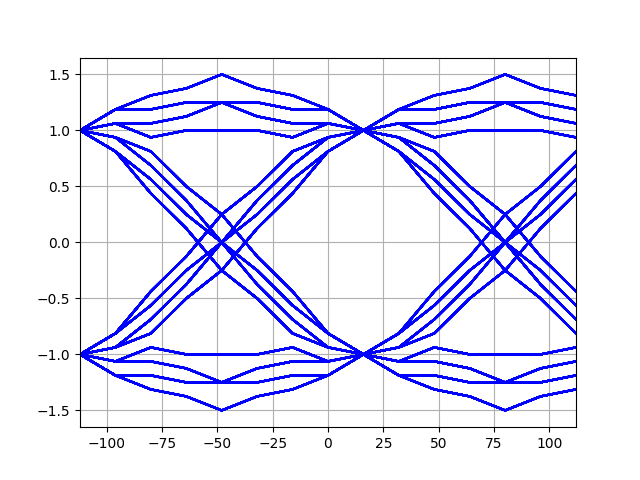
\includegraphics[width=\linewidth]{imagenes_FP/eye_d_filter1q6,4_round.png}
    \end{subfigure}
    \caption{Diagrama de ojo S(6,4) rounded con $\alpha=0.5$}
    \label{fig:eye_d_filter1q6_4_round}
\end{figure}

\begin{figure}[H]
    \centering

    \begin{subfigure}{0.49\textwidth}
        \centering
        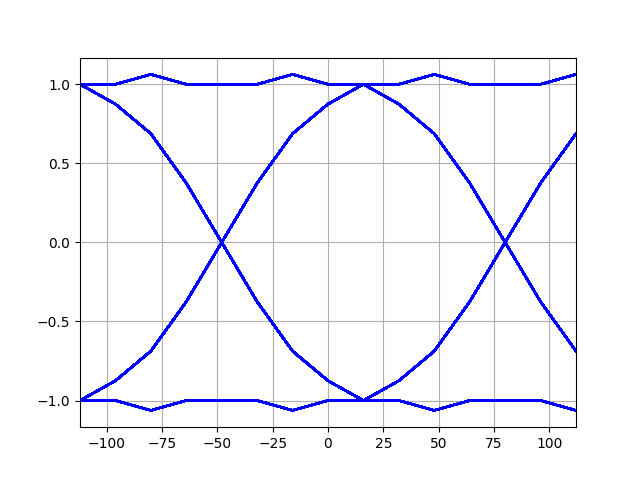
\includegraphics[width=\linewidth]{imagenes_FP/eye_d_filter2i6,4_round.png}
    \end{subfigure}
    \hfill
    \begin{subfigure}{0.49\textwidth}
        \centering
        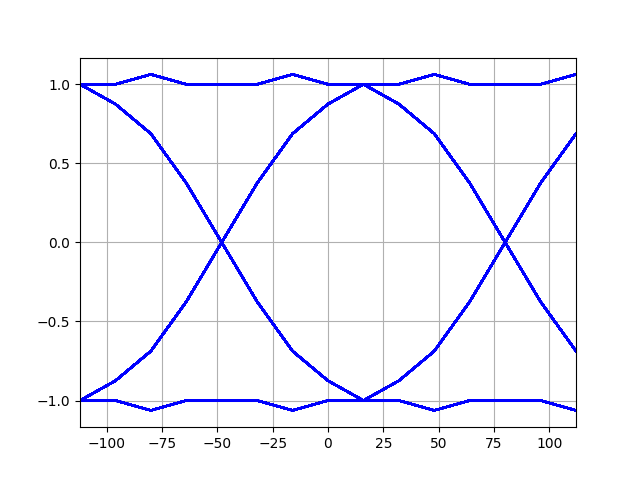
\includegraphics[width=\linewidth]{imagenes_FP/eye_d_filter2q6,4_round.png}
    \end{subfigure}
    \caption{Diagrama de ojo S(6,4) rounded con $\alpha=1$}
    \label{fig:eye_d_filter2q6_4_round}
\end{figure}

\begin{figure}[H]
    \centering

    \begin{subfigure}{0.32\textwidth}
        \centering
        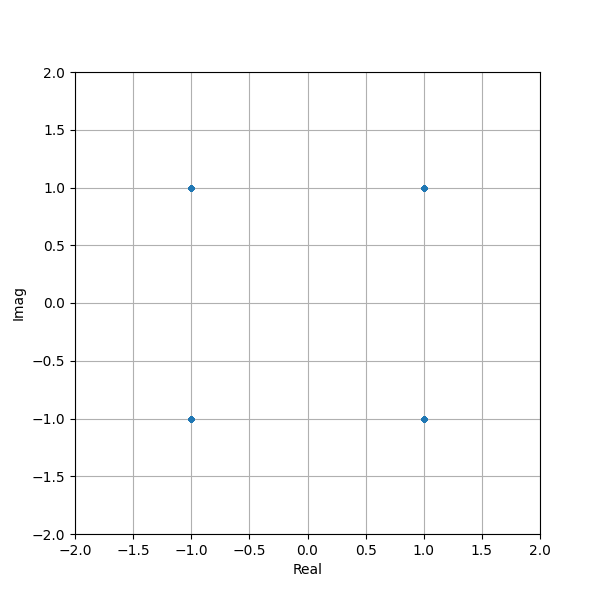
\includegraphics[width=\linewidth]{imagenes_FP/constelation_filters_opt6,4_round.png}
        \caption{$\alpha=0$}
    \end{subfigure}
    \hfill
    \begin{subfigure}{0.32\textwidth}
        \centering
        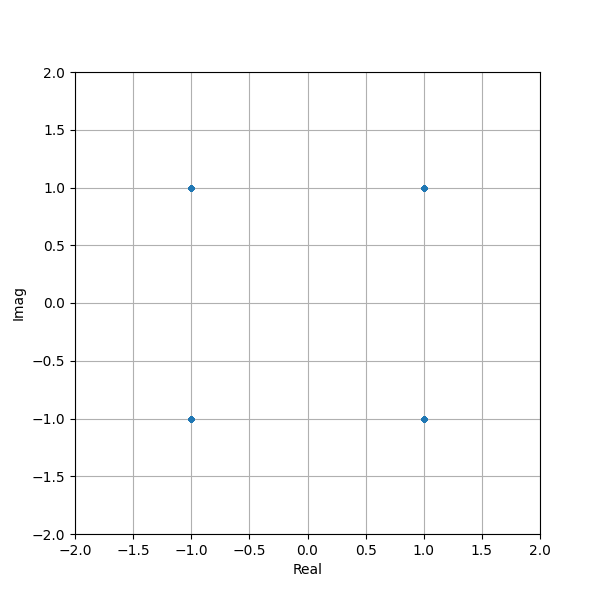
\includegraphics[width=\linewidth]{imagenes_FP/constelation_filters_opt6,4_round.png}
        \caption{$\alpha=0.5$}
    \end{subfigure}
    \hfill
    \begin{subfigure}{0.32\textwidth}
        \centering
        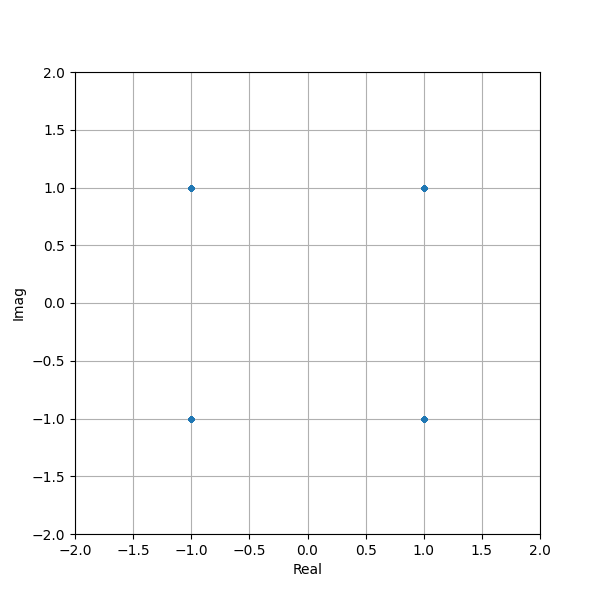
\includegraphics[width=\linewidth]{imagenes_FP/constelation_filters_opt6,4_round.png}
        \caption{$\alpha=1$}
    \end{subfigure}
    \caption{Constelaciones según $\alpha$ para S(6,4) rounded}
    \label{fig:constelations_filters_opt6_4_round}
\end{figure}

\subsection{Diferencias entre cuantizaciones}

En esta sección se analizarán las \textbf{ventajas y desventajas} obtenidas para cada una
de las cuantizaciones realizadas, observando todos los gráficos obtenidos y comparándolos
entre si para ver cuál es el más óptimo para una comunicación normalizada.

Para comenzar, resaltando lo obvio, fue muy importante la cantidad de bits a utilizar para la cuantización.
Esta selección de bits tendrá un papel fundamental en la calidad de la señal recibida.

Los principales prospectos que muestran esta diferencia son las \textbf{cuantizaciones S(3,2) y S(8,7)}, donde se
puede ver con claridad en las figuras \ref{fig:rta_imp_3_2_trunc} y \ref{fig:rta_freq_3_2_trunc}, donde prácticamente
no se puede distinguir el ruido de los símbolos enviados sin importar si se utiliza truncado o redondeo, como lo muestran las figuras
\ref{fig:rta_imp_3_2_round} y \ref{fig:rta_freq_3_2_round}.

El diagrama de ojo y la constelación de la \textbf{cuantización S(3,2)} también muestran un importante
aspecto en el análisis; En las figuras \ref{fig:constelations_filters_opt3_2_trunc} y \ref{fig:constelations_filters_opt3_2_round}
se observa que la selección entre el redondeo y el truncado tiene un papel clave en la minimzación de la ISI.

Se puede reforzar esta conclusión en la \textbf{cuantización S(8,7)}, donde en las figuras
\ref{fig:constelations_filters_opt8_7_trunc} y \ref{fig:constelations_filters_opt8_7_round} se observa
la minimización de la ISI en las constelaciones por el efecto del redondeo.

Por último, la cuantización más equilibrada fue la \textbf{S(6,4)}, donde la cantidad de bits es la justa
como para representar fielmente los símbolos enviados, como se puede ver en las figuras \ref{fig:simbols_in_out6_4_round} y \ref{fig:simbols_in_out6_4_trunc}. Donde
los símbolos recibidos pueden reconocerse en gran medida, aunque no tan bien como en la \textbf{cuantización S(8,7)}. Esto se debe a que, aunque la cantidad de bits 
totales no sea tan diferente, sí lo es la cantidad de bits fraccionarios, siendo casi el doble en la segunda. De igual manera, 
la relación entre la cantidad de bits enteros también cambia, lo que hace que se pierda aún más calidad.

Esto se puede mejorar manteniendo la relación de bits enteros, es decir, utilizando una \textbf{cuantización S(6,5)}

En lo que respecta al redondeo, la ISI nuevamente se vuelve nula en los coeficientes redondeados, como se ve en la figura \ref{fig:constelations_filters_opt6_4_round}

Se confeccionó un cuadro resumen para mejorar la comparación de cada cuantización.

\begin{table}[h]
    \centering
    \caption{Rendimiento según el tipo de Cuantización}
    \label{tab:tabla_cuantizaciones}
    \begin{tabularx}{\textwidth}{lXXX}
        \toprule
        \textbf{Estrategia} & \textbf{S(8,7)} & \textbf{S(6,4)} & \textbf{S(3,2)} \\
        \midrule
        Redondeo &
        -ISI nula. \newline
        -Buena cantidad de bits. Respuesta casi perfecta \newline
        -Mayor cómputo.
        &
        -ISI nula. \newline
        -Respuesta fiel pero inexacta. \newline
        -Cómputo intermedio.
        &
        -ISI nula pero constelación desplazada. \newline
        -SNR baja. \newline
        -Cómputo bajo.
        \\
        \midrule
        Truncado &
        -Muy poca ISI. \newline
        -Buena cantidad de bits, respuesta aceptable. \newline
        -Cómputo intermedio.
        &
        -ISI significativa. \newline
        -Cantidad de bits inefectiva para truncar. \newline
        -Cómputo muy bajo.
        &
        -ISI destructiva. \newline
        -SNR muy baja. \newline
        -Cómputo minimizado.
        \\
        \bottomrule
    \end{tabularx}
\end{table}
\newpage


\section{Conclusiones}

Finalizando con el informe, se concluye que, para cada caso de cuantización, es muy importante
tener en cuenta los recursos de cómputo que se poseen para seleccionar la
cuantización correcta.
En este trabajo se vio como el efecto del error de cuantización nos obliga a jugar con el
equilibrio entre procesamiento y fidelidad, como ocurre con otros aspectos del área del DSP,
como ser el manejo del Timing o de la potencia.

También fue clave entender el uso de los diagramas de ojo y
las constelaciones para poder verificar el correcto funcionamiento de la transmisión de datos entre
módulos.
\end{document}
